\section{Ongoing Research Efforts and Challenges}
\label{sec:challenges}


The research \coloredtext{developments} we have surveyed so far seek to overcome the challenges of realizing the vision and fulfilling the \coloredtext{promises} of SDN.
While Section~\ref{sec:layeredapproach} provided a perspective structured across the layers of the ``SDN stack'', this
section highlights research \coloredtext{efforts} we consider of particular importance for unleashing the full potential of SDN, and that therefore deserves a specific coverage in this survey.

\begin{comment}

Scalability, security and dependability, organizational barriers,
migration, minimally standardized northbound APIs, and global-scale
network services can be considered as some of the main challenges of
SDNs.  Despite  several works that address different scaling
issues in software-defined networks, scalability still needs attention
in large-scale enterprise
deployments~\cite{yeganeh2013,Li:2012:Toward:0001,yu2010-1}.  For
instance, one of the fundamental demanding features of distributed
network operating systems is consistent data distribution and fault
tolerance.  In control platforms designs the performance penalty for
strong data consistency among controller nodes is significantly
high~\cite{koponen-1}.
%However, recent research have shown that high performance of fault tolerant and strongly consistent data stores for distributed SDN control platforms is an achievable goal~\cite{botelho2013}.
Furthermore, cellular networks, first class data centers and
backbones, are three examples of challenging large-scale  scenarios for SDNs.

Security and dependability are first class priorities of any network architecture, and especially critical for control split approaches as in SDN.
In particular, enterprise deployments demand higher levels of security
and dependability, in order to give the appropriate confidence guarantees to infrastructure stakeholders~\cite{sorensen2012,kerner2013}.
In fact, currently available SDN standards and solutions provide only a few basic  features and properties with respect to security and dependability, such as encrypted TLS channels, flow rate limits, and master/slave controllers to tolerate failures.
However, as will be shown in the following sections, this is far from enough to mitigate most of the existing threats.

Examples of challenges regarding organizational barriers, migration, minimally standardized northbound APIs, and global-scale network services will also be explored throughout the section.
For instance, differently from storage and computing resources, which are nearly globally available through cloud providers, infrastructures that provide flexible Network-as-a-Service are still far from reality.
Despite the fact that SDN brings new means and opportunities, there is a long path to go and many difficulties to overcome, such as how to create cross domain virtual networks with quality of service and quality of protection guarantees.

\end{comment}

%IMplementation challenges:
%http://ieeexplore.ieee.org/xpl/articleDetails.jsp?arnumber=6553676

\subsection{Switch Designs}

% ~\cite{rotsos2012-1,wundsam2012,huang2013}
Currently available OpenFlow switches are very diverse and exhibit notable differences in terms of 
feature set (e.g., flow table size,  optional actions), performance (e.g., fast vs. slow 
path, control channel latency/throughput), interpretation and adherence to the protocol 
specification (e.g., \texttt{BARRIER} command), and architecture (e.g., hardware vs. software designs).

%\subsubsection{Heterogenous Implementations}
\vspace{2mm}
\noindent \textit{Heterogenous Implementations}

Implementation choices have a fundamental impact on the behavior, accuracy, and performance of switches, 
ranging from differences in flow counter behavior~\cite{curtis2011} to a number of 
other performance metrics~\cite{rotsos2012-1}. One approach to accommodate such heterogeneity 
is through NOSIX, a portable API that separates the application expectations from the switch heterogeneity~\cite{wundsam2012}. To do so, NOSIX provides a pipeline of multiple virtual flow 
tables and switch drivers. Virtual flow tables are intended to meet the expectations of applications and 
are ultimately translated by the drivers into actual switch flow tables. 
Towards taming the  complexity of multiple OpenFlow protocol versions with different sets of required and optional capabilities, a roadblock for SDN practitioners, tinyNBI~\cite{casey2014} has been proposed as a  simple API providing a unifying set of core abstractions of five OpenFlow protocol versions (from 1.0 to 1.4).
Ongoing efforts to introduce a new Hardware Abstraction Layer  (HAL) for non-OpenFlow capable devices~\cite{alienfp7}  include the development of open source artifacts like ROFL (Revised OpenFlow Library) and the xDPd (eXtensible DataPath daemon), a framework for creating new OpenFlow datapath implementations based on a diverse set of hardware and software platforms.
A related open source effort to develop a common library to implement OpenFlow 1.0 and 1.3 protocol endpoints (switch agents and controllers) is libfluid~\cite{libfluid}, winner of the OpenFlow driver competition organized by the ONF.

Within the ONF, the Forwarding Abstraction Working Group (FAWG) is pursuing another solution to the heterogeneity problem, through Table Type Patterns 
(TTPs)~\cite{onf2013}. A TTP is a standards-based and negotiated switch-level behavioral abstraction. 
It consists of the relationships between tables forming a graph structure, the types of tables in the graph, 
a set of the parameterized table properties for each table in the graph, the legal \texttt{flow-mod} and \texttt{table-mod} commands for 
each flow table, and the metadata mask that can be passed between each table pair in the graph. 


%\subsubsection{Flow Table Capacity}
\vspace{2mm}
\noindent \textit{Flow Table Capacity}

Flow matching rules are stored in flow tables inside network devices.
One practical challenge is to provide switches with large and efficient flow tables to store the 
rules~\cite{appelman2012}. TCAMs are a common choice to hold flow tables. While flexible 
and efficient in terms of matching capabilities, TCAMs are costly and usually small (from 4K to 32K 
entries). Some TCAM chips today integrate 18 M-bit (configured as 500k entries $*$ 36 bit per entry) 
into a single chip working at 133 Mhz~\cite{kannan2013}, i.e., capable of 133M lookups 
per second. However, these chips are expensive and have a high-power consumption~\cite{liao2012}, 
representing a major power drain in a switching device~\cite{agrawal2006}. These are some of the reasons 
why currently available OpenFlow devices have TCAMs with roughly 8K entries, where the actual capacity 
in terms of OpenFlow table size has a non-trivial relationship to the type of flow entries being used~\cite{owens2013,salisbury2012}. OpenFlow version 1.1 introduced multiple tables, 
thereby adding extra flexibility and scalability. Indeed, OpenFlow 1.0 implied state explosion due to 
its flat table model~\cite{onf2013}. However, supporting multiple tables in hardware is challenging 
and limited -- yet another motivation for the ongoing ONF FAWG work on TTPs~\cite{onf2013}.

\coloredtext{Some efforts focus on compression techniques to reduce the number of flow entries in TCAMs~\cite{Braun2014,Agarwal2014_42,Rudell1987espresso}.
The Espresso heuristic~\cite{Rudell1987espresso} can be used to compress wildcards of OpenFlow-based inter-domain routing tables, reducing the forwarding information base (FIB) by 17\% and, consequently, saving up to 40,000 flow table entries~\cite{Braun2014}. 
Shadow MACs~\cite{Agarwal2014_42} propose label switching for solving two problems, consistent updates and rule space exhaustion, by using opaque values (similar to MPLS labels) to encode fine-grained paths as labels. 
A major benefit of fixed-size labels is relying on exact-math lookups which can be easily and cost-effectively implemented by simple hardware tables instead of requiring rules to be encoded in expensive TCAM tables.

%As an example, large L2 forwarding tables (e.g., 100,000+ entries), which are common in forwarding devices, can be used to install shadow MAC forwarding rules.
%Such solutions represent promising opportunities for further investigation towards solving the problem of TCAM size by a variety of means.
}

%\subsubsection{Performance}
\vspace{2mm}
\noindent \textit{Performance}

\coloredtext{Today, the throughput of commercial OpenFlow  switches varies from 38 to 1000 \texttt{flow-mod} per second, with most devices achieving a throughput lower than 500 \texttt{flow-mod} per second~\cite{Bifulco2014, stephens2012-1}.}
This is clearly a limiting 
factor that shall be addressed in the switch design process -- support of OpenFlow in existing product 
lines has been more a retrofitting activity than a clean feature planning and implementation activity. Deployment experiences~\cite{Kobayashi2014151} have pointed to a series of challenges stemming from the limited embedded CPU power of current commercial OpenFlow switches. 
One approach to handle the problem consists of adding more powerful CPUs into the switches, as proposed 
in~\cite{mogul2012}. Others have proposed to rethink the distribution of control 
actions between external controllers and the OpenFlow agent inside the switch~\cite{curtis2011}. 
Our current understanding indicates that an effective way forward is a native design of SDN switches 
consistent with the evolution of the southbound API standardization activities~\cite{bosshart2013-1,onf2013}. 

% Note: NetVM~\cite{hwang2014} is an approach for high performance, line rate, within new technologies such as DPDK~\cite{intelcorporation2014}.

\coloredtext{
%\subsubsection{Evolving Switch Designs}
\vspace{2mm}
\noindent \textit{Evolving Switch Designs \& Hardware Enhancements}

As in any soft\-wa\-re/hard\-wa\-re innovation cycle, a number of advancements are to be expected from the hardware 
perspective to improve SDN capabilities and performance. 
New SDN switch designs are appearing in a myriad of hardware 
combinations to efficiently work together with TCAMs, such as SRAM, RLDRAM, DRAM, GPU, FPGA, NPs, CPUs, 
among other specialized network processors~\cite{ferkouss2011,naous2008,memon2013,luo2009,rostami2012,pongracz2013}.} These early works suggest the need for additional efforts into new hardware architectures for future 
SDN switching devices. For instance, some proposals target technologies such as GPUs that have demonstrated 
20 Gbps with flow tables of up to 1M exact match entries and up to 1K wildcard entries~\cite{memon2013}. 
Alternatives to TCAM-based designs include new hardware architectures and components, as well as new and more 
scalable forwarding planes, such as the one proposed by the Rain Man firmware~\cite{stephens2012}.
Other design solutions, such as parallel lookup models~\cite{li2013}, can also be applied to SDN to reduce 
costs in switching and routing devices. Recent proposals on cache-like OpenFlow switch arrangements~\cite{katta2013} shed some light on overcoming the practical limitations of 
flow table sizes with clever switching designs. Additionally, counters represent another practical challenge 
in SDN hardware implementations. Many counters already exists, and they could lead to significant control 
plane monitoring overhead~\cite{curtis2011}. Software-defined counters 
(SDC)~\cite{mogul2012} have been proposed to provide both scalability and flexibility.

%As most of the current SDN switches and protocols are limited to inspect header fields of layers 2, 3 and 4, customized handling, requiring information of higher layers, has to be done in the control plane.
%To overcome this limitation, 
\coloredtext{
Application-aware SDN architectures are being proposed to generalize the standard OpenFlow forwarding abstractions by including stateful actions to allow processing information from layers 4 to 7~\cite{Mekky2014-4}.
%However, this implies redesigning the data plane devices. 
%, as has already been demonstrated using an extended version of the Open vSwitch.
%Instead of having only traditional flow tables, 
%in order to support stateful application-aware actions, 
%forwarding devices should support kernel flow tables, user flow tables, and application flow tables~\cite{Mekky2014-4}.
To this end, application flow tables are proposed as data plane application modules that require only local state, i.e., do not depend on a global view of the network. Those tiny application modules run inside the forwarding devices (and can be installed on-demand), alleviating the overhead on the control plane and augmenting the efficiency of certain tasks, which can be kept in the data plane. 
Similarly, other initiatives propose solutions based on pre-installed state machines.
FAST (Flow-level State Transitions)~\cite{Moshref2014_4} allows controllers to proactively program state transitions in forwarding devices, allowing switches to run dynamic actions that require only local information.
%Such solutions reduce the burden of the control plane and give more power to application developers to decide what actions should be kept in the data plane in order to improve the network efficiency regarding the task of processing flows.

Other approaches towards evolving switch designs include CAching in Buckets (CAB), a reactive wildcard caching proposal that uses a geometric representation of the rule set, which is divided into small logical structures (buckets)~\cite{Yan2014CAB}. 
Through this technique CAB is able to solve the rule dependency problem and achieve efficient usage of control plane resources, namely bandwidth, controller processing load, and flow setup latency.
 
New programmable Ethernet switch chips, such as XPliant Ethernet~\cite{McGillicuddy2014_4}, are emerging into this new market of programmable networks.
Its main aim is enabling new protocol support and the addition of new features through software updates, increasing flexibility.
%This means that it introduces a remarkable flexibility into the market, fostering innovation at a faster pace.
One example of such flexibility is the support of GENEVE~\cite{Gross2014_4}, a recent effort towards generic network virtualization encapsulation protocols, and OpenFlow.
% which allows switch vendors to add support to new protocols through software updates. % and make it rapidly available for its customers.
The throughput of the first family of XPliant Ethernet chip varies from 880 Gbps to 3.2 Tbps, supporting up to 64 ports of 40 GbE or 50 GbE, for instance. 
%Such kind of new technologies, coming into the market, have the potential of boosting the research and development of new switching devices with several features that allow the development and deployment of new generations of SDN-enabled forwarding devices.
}


%\subsubsection{Hardware Enhancements/Support}
%\vspace{2mm}
%\noindent \textit{Hardware Enhancements \& Support}

%As in any soft\-wa\-re/hard\-wa\-re innovation cycle, a number of advancements can be expected from the hardware 
%perspective to improve SDN capabilities and performance~%\cite{intelprocessors2012,brebner2012,appelman2012,matsumoto2012,naous2008,bianco2010}.
Microchip companies like Intel are already shipping processors with flexible SDN capabilities to the 
market~\cite{intelprocessors2012}. Recent advances in general-purpose CPU technology include a
data-plane development kit~(DPDK)~\cite{intelcorporation2014} that allows high-level programming of how data 
packets shall be processed directly within network interface cards. Prototype implementations of Intel 
DPDK accelerated switch shows the potential to deliver high-performance SDN software switches~\cite{pongracz2013}. This trend is likely to 
continue since high-speed and specialized hardware is needed to boost SDN performance and scalability for 
large, real-world networks. Hardware-programmable technologies such as FPGA are widely used to reduce time 
and costs of hardware-based feature implementations. NetFPGA, for instance, has been a pioneering technology 
used to implement OpenFlow 1.0 switches~\cite{naous2008}, providing a commodity 
cost-effective prototyping solution. Another line of work on SDN data planes proposes to augment switches 
with FPGA to (remotely) define the queue management and scheduling behaviour of packet 	
switches~\cite{sivaraman2013}.
\coloredtext{
Finally, recent developments have shown that state-of-the-art System-on-chip (SoC) platforms, such as the Xilinx Zynq ZC706 board, can be used to implement OpenFlow devices yielding 88 Gpbs throughput for 1K flow supporting dynamic updates~\cite{Zhou2014-4}. 
%This is undoubtedly another example of a research direction for overcoming some of the challenges faced by current OpenFlow-enabled forwarding devices.
}

%\subsubsection{Native SDN Switch Designs}
\vspace{2mm}
\noindent \textit{Native SDN Switch Designs}

Most of the SDN switch (re)design efforts so far follow an evolutionary approach to retrofit 
OpenFlow-specific programmable features into existing hardware layouts, following common wisdom 
on switch/router designs and consolidated technologies (e.g., SRAM, TCAM, FPGA). One departure from 
this approach is the ongoing work on \textit{forwarding metamorphosis}~\cite{bosshart2013-1}, 
a reconfigurable match table model inspired from RISC-like pipeline architecture applied to switching 
chips. This work illustrates the feasibility of realizing a minimal set of action primitives for flexible 
header processing in hardware, at almost no additional cost or power. Also in line with the core SDN goals 
of highly flexible and programmable (hardware-based) data planes, Protocol-Oblivious Forwarding (POF)~\cite{song2013-1} aims at overcoming some of the limitations of OpenFlow (e.g., expressiveness, 
support of user-defined protocols, memory efficiency), through generic flow instruction sets.
Open-source prototypes are available~\cite{song2013} as well as evaluation 
results showing the line-speed capabilities using a network processing unit (NPU)-based~\cite{Hauger2009} proof of concept implementation. 
\coloredtext{In this line, we already mentioned OpenState~\cite{bianchi2014}, another initiative that aims to augment the capability and flexibility of forwarding devices. 
By taking advantage of eXtended Finite State Machines (XFSM)~\cite{bianchi2012,tinnirello2012}, OpenState proposes an abstraction -- as a super set of OpenFlow primitives -- to enable stateful handling of OpenFlow rules inside forwarding devices. 
%Speaking differently, this is an example of how alternative approaches can be further explored to provide powerful capabilities to the forwarding devices without impairing on the  decoupling of the control and data planes. 
}

In the same way as TTPs allow controllers to compile the right set of low-lever instructions known to be supported by the switches, a new breed of switch referred to as P4 (programmable, protocol-independent packet
processor)~\cite{bosshart2013} suggests an evolution path for OpenFlow, based on a high-level compiler. 
This proposal would allow the functionality of programmable switches (i.e., pipeline, header parsing, field matching) to be not only specified by the controller but also changed in the field.
In this model, programmers are able to decide how the forwarding plane processes packets without caring about implementation details.
It is then the compiler that transforms the imperative program into a control flow graph that can be mapped to different target switches. 

% http://conferences.sigcomm.org/sigcomm/2013/papers/hotsdn/p127.pdf

% Fast Programmable Match-Action Processing in Hardware for SDN
%On the cost and speed:
%\begin{itemize}
%\item Single Match Table: costly and wastful
%\item Multiple Match Tables: severely limits flexibility and limited repertoire of actions corresponding to common processing behaviors
%\item Reconfigurable Match Tables: allows a set of pipeline stages and four ways of data plane reconfigurability
%\end{itemize}


%OpenPipes: Prototyping high-speed networking systems~\cite{gibb2009}
%Build and connect high performance modules via OpenFlow network...

%
%ServerSwitch: A Programmable and High Performance Platform for Data Center Networks~\cite{lu2011}
%
%Stochastic Switching Using OpenFlow~\cite{shourmasti2013}
%
%ITEM hardware architectures, devices and performance ... ~\cite{intelprocessors2012,brebner2012,appelman2012,matsumoto2012,naous2008,bianco2010}
%
%ITEM Switch implementation and performance issues... ~\cite{rotsos2012-1,bianco2010,curtis2011,yu2010-1};
%
%There are several challenges related to the forwarding plane performance~\cite{rotsos2012-1,bianco2010,curtis2011,yu2010-1}.
%
%
%
%Towards TCAM-based Scalable Virtual Routers~\cite{luo2012}
%
%
%Accelerating OpenFlow Switching with Network Processors~\cite{luo2009}
%
%A 100Gig network processor platform for openflow~\cite{ferkouss2011}
%
%FlashFlow: a GPU-based Fully Programmable OpenFlow Switch~\cite{memon2013}
%Goal: reach 20 Gbps with flow tables of up to 1M exact match entries and up to 1K wildcard entries.
%
%\note{DK ... 
%    In some earlier work ~\cite{das2011-1}, authors apply network processor based acceleration cards to perform OpenFlow switching. They propose and describe the design options and report re- sults that show a 20\% reduction on packet delay. Also, in ~\cite{Yap:2010:TSN:1851276.1851288}, an architectural design to improve look-up performance of OpenFlow switching in Linux is proposed. Preliminary results reported show a packet switching throughput increase up to 25\% compared to the throughput of regular software-based OpenFlow switching. Another study on dataplane performance over Linux based OpenFlow switching is presented in ~\cite{foster2011}.
%}


\subsection{Controller Platforms}

In the SDN model, the controller platform is a critical pillar of the architecture, and, as such, 
efforts are being devoted to turn SDN controllers into high-performance, scalable, distributed, 
modular, and highly-available programmer-friendly software.
\coloredtext{Distributed controller platforms, in particular, have to address a variety of challenges. 
Deserving special consideration are the latency between forwarding devices and controller instances,  fault-tolerance, load-balancing, consistency and synchronization,  
%SDN providers with a geographically local footprint, 
among other issues~\cite{koponen-1,schmid2013,Berde2014ONOS}.
Operators should also be able to observe and understand how the combination of different functions and modules can impact their network~\cite{Volpano2014_4}.
%This concern is regarding all control platforms, i.e., different mixing of functions and modules can result in unexpected network behaviors, ranging from simple things such as an overhead on control plane latency to the disruption of certain functionalities (i.e., introduce bugs in the network).
%In spite of the importance of those issues, most of them are still open avenues, requiring further investigation and development.
}

%\begin{itemize}
%\item Distribution:
%\item Elasticity:
%\item Architecture:
%\item Orchestration:
%\item Modularity:
%\end{itemize}

%\vspace{2mm}
%\noindent \textit{Performance}

As the SDN community learns from the development and operational experiences with OpenFlow controllers (e.g., Beacon~\cite{erickson2013}), further advancements are expected in terms of raw performance of controller implementations, including the exploitation of hierarchical designs and optimized buffer sizing~\cite{azodolmolky2013-2}.  
\coloredtext{One approach to increase the performance of controllers is the IRIS IO engine~\cite{Park2014}, enabling  significant increases %(e.g., 26\%)
in the flow-setup rate of SDN controllers. 
Another way of reducing the control plane overhead is by keeping a compressed copy of the flow tables in the controller's memory~\cite{zhang2014-4}.
%However, one of the major challenges of such approaches is to reduce the flow table size in memory.
%Early experimental results show that model-based compression methods can help to efficiently store, compress (up to 98\%) and keep a copy of flow tables in memory~\cite{zhang2014-4}, which helps to reduce the number of messages between controllers and forwarding devices, as well as improve the recovery efficiency in case of failures.
%Once the controller knows the flow table state of all forwarding devices, on case of any data plane disruption, configurations can be rapidly and straightforward reseted on the devices, when even necessary.
}
%A more detailed discussion on performance evaluation will be presented in Section~\ref{sec:performance-eval}. 
%While the first commercially available controllers supporting OpenFlow 1.3 are capable of handling up to 200 physical switches per controller and/or 10.000 ports~\cite{little2013}, we expect these numbers to be transient

%Performance Evaluation of a Scalable Software-Defined Networking Deployment
%Given these parameters, the required buffer size of the root SDN controller amounts to 0.83 million events in worst case scenario. This result helps the designers provision the required buffer space (i.e., buffer sizing

% Modularity
%\subsubsection{Modularity}
\vspace{2mm}\coloredtext{
\noindent \textit{Modularity \& Flexibility}}

\coloredtext{A series of ongoing research efforts target the modular and flexible composition of controllers. 
RAON~\cite{Park2014-1} proposes a recursive abstraction of OpenFlow controllers where each controller sees the controllers below as OpenFlow switches. %, i.e., not implying in major changes or adaptations on the current SDN/OpenFlow model. 
%While major changes or adaptations on the current SDN/OpenFlow model. 
%Concerns such as the overhead in terms of control messages, overall flexibility and simplicity have still to be further investigated.
Open research issues include the definition of suitable interfaces between the different layers in such a hierarchy of controllers. % have not yet been deeply enough researched or understood. 
%Approaches similar to RAON~\cite{Park2014-1} are considering the current southbound APIs as the main means for communicating between levels of controllers. 

Other open issues to be further investigated in this context are the East/westbound APIs, and their use in enabling suitable hierarchical designs to achieve scalability, modularity, and security~\cite{ONF2014SDNarch}. 
For instance, each level of a hierarchy of controllers can offer different abstractions and scopes for either intra- and inter-data center routing, thus increasing scalability and modularity.
%Yet, this can be hard to achieve with low-level southbound APIs, like OpenFlow, as the main communication interface between different levels of controllers.
Similarly, from a security perspective, each hierarchical level may be part of a different trust domain.
Therefore, east/westbound interfaces between the different layers of controllers should be capable of enforcing both intra- and inter-domain security policies.
%These are some of the open issues to be further investigated on the context of hierarchies of controllers, in both intra- and inter-domain use cases

Another important observation is that, currently, the lack of modularity in most SDN controllers forces developers to re-implement basic network services from scratch in each new application~\cite{Casado2014_4}. 
%Consequently, modularity is becoming one of the major requirements in SDN for the future development and sustainability of the controllers' ecosystem.
%Application developers need to be able to easily build applications from existing services and functions, implementing only new services.
%Composition and isolation (e.g., applications running as processes similarly to what happens in traditional operating systems) will play important rules on the development of the new generations of network operating systems.
} 
As in software engineering in general, lack of modularity results in controller 
implementations that are hard to build, maintain, and extend -- and ultimately become resistant to further 
innovations, resembling traditional ``hardware-defined'' networks. As surveyed in Section~\ref{sec:programminglanguages}, 
SDN programming abstractions (e.g.,~Pyretic~\cite{monsanto2013}) introduce modularity in SDN 
applications and simplify their development altogether. Further research efforts (e.g., 
Corybantic~\cite{auyoung2013}) try to achieve modularity in SDN control programs. Other 
contributions towards achieving modular controllers can be expected from other areas of computer science 
(e.g., principles from Operating System~\cite{monaco2013}) and best practices of modern 
cloud-scale software applications.


%\subsection{Data Plane Performance}
%
%NetVM~\cite{hwang2014}
%ClickOS~\cite{martins2014}
\vspace{2mm}
\noindent \textit{Interoperability and application portability}

Similarly to forwarding device vendor agnosticism that stems from standard southbound interfaces, it is important to foster interoperability between controllers.
Early initiatives towards more interoperable control platforms include portable programming languages such as Pyretic~\cite{monsanto2013} and east/westbound interfaces among controllers, such as SDNi~\cite{yin2012}, ForCES CE-CE interface~\cite{doria2010,wang2011-1}, 
and ForCES Intra-NE mechanisms~\cite{ogawa2013}.
However, these efforts are yet far from fully realizing controller interoperability and application portability.
%The next chapters of SDN will give a better idea of what is going to happen regarding these important issues for the heathy development of an open market of paramount importance, i.e., the control platform ecosystem.

\coloredtext{
In contrast to Pyretic~\cite{reich2013}, PANE~\cite{ferguson2013},
Maple~\cite{voellmy2013}, and Corybantic~\cite{auyoung2013}, which are
restricted to traffic engineering applications and/or impose
network state conflict resolution at the application level (making
application design and testing more complicated),
Statesman~\cite{Sun2014nms} proposes a framework to enable a
variety of loosely-coupled network applications to co-exist on the
same control plane without compromising network safety and
performance.
This framework makes application development simpler by automatically and transparently resolving conflicts.
In other words, Statesman allows a safe composition of uncoordinated
or conflicting application's actions. 
%through an abstraction of three distinct views of the network, observed state, proposed state and target state. 
%While applications read the observed state and propose a new value for
%state variables, the Statesman framework uses a dependency model to
%merge the proposed states into a reliable target state.
%In case of conflicts, Statesman supports two mechanisms,
%last-writer-wins and highest-priority-wins.
%Experimental results have shown that last-writer-wins mechanisms is
%good enough since corner cases are unlikely to happen, i.e., two
%applications (with distinct priorities) competing for the same state
%variable at the same time.
%Therefore, Statesman is a good example of a solution, as well as a research
%direction, to foster the development of control platforms capable of
%supporting a wider variety of loosely-coupled applications without
%impairing safety and performance.
}

\coloredtext{
Another recent approach to simplify network management is the idea of compositional SDN hypervisors~\cite{Jin2014_4}.
Its main feature is allowing applications written in different languages, or on different platforms, to work together in processing the same traffic.
The key integration component is a set of simple prioritized lists of OpenFlow rules, which can be generated by different programming languages or applications. 
%This is one of the early examples of how hypervisors can also become useful tools for promoting interoperability and portability in this rather diverse ecosystem of control platforms.
}

%\subsubsection{High Availability}
% Production quality, HA
\vspace{2mm}
\noindent \textit{High-Availability}

In production, SDN controllers need to sustain healthy operation 
under the pressure of different objectives from the applications they
host. Many advances are called for in order
to deal with potential risk vectors of controller-based solutions~\cite{kreutz2013}. Certainly, 
many solutions will leverage on results from the distributed systems and security communities made over the last decade. 
\coloredtext{For instance, recent efforts propose consistent, fault-tolerant data stores for building reliable distributed controllers~\cite{botelho2013,Botelho2014,Berde2014ONOS}.
}

\coloredtext{Another possible approach towards building low latency, highly available SDN controllers is to exploit controller locality~\cite{schmid2013,levin2012}.
Classical models of distributed systems, such as LOCAL and CONGEST~\cite{Peleg2000}, can be explored to solve this problem.
Those models can be used to develop coordination protocols that enable each controller to take independent actions over events that take place in its local neighborhood~\cite{schmid2013}. 
}

\coloredtext{Another core challenge relates to the fundamental trade-offs between the consistency model of state distribution in distributed SDN controllers, the consistency requirements of control applications, and performance~\cite{levin2012}.
%These trade-offs results in challenges associated to the complexity of the application logic and the persistency and robustness of the state kept by the NOS. 
%The main issue is related to applications that are unaware of the potential effects of its own logic according to the state provided by the underlying SDN controller. 
%In an ideal scenario, 
To ease development, the application should ideally not be aware of the vagaries of distributed state.
This implies a strong consistency model, which can be achieved with distributed data stores as proposed recently~\cite{botelho2013}.
However, keeping all control data in a consistent distributed data store is unfeasible due to the inherent performance penalties.
Therefore, hybrid solutions are likely to co-exist requiring application developers to be aware of the trade-offs and penalties of using, or not, a strong consistency model, a tenet of the distributed Onix controller~\cite{koponen-1}. 
%While it can be very useful in many situations, it might not be necessary in other cases, where decisions can be make by applications without necessarily having a consistent global network view.
}

\coloredtext{High availability can also be achieved through improved southbound APIs and controller placement heuristics and formal models~\cite{Ros2014_4,philip2014cross, Borokhovich2014_4}. These aim to maximize resilience and scalability by allowing forwarding devices to connect to multiple controllers in a cost-effective and efficient way~\cite{philip2014cross}.
Early efforts in this direction have already shown that forwarding devices connecting to two or three controllers can typically achieve high availability (up to five nines) and robustness in terms of control plane connectivity~\cite{Ros2014_4,Borokhovich2014_4}.
It has also been shown that the number of required controllers is more dependent on the topology than on network size~\cite{Ros2014_4}.
Another finding worth mentioning is the fact that for most common topologies and network sizes fewer than ten controllers seem to be enough~\cite{Ros2014_4}. 
%Nevertheless, in this direction there is still room for further investigation and developments.
%Currently, SDN control planes and most control platforms still lack mechanisms and architectural enhancements for achieving the practical availability and reliability levels required for enterprise deployments.
}

%%% autoscaling paper



%\coloredtext{
%\vspace{2mm}
%\noindent \textit{Heterogeinity \& Diversity}
%
%The ecosystem of controllers needs also another important ingredient, which is heterogeneity in the sense that different controller architectures may be necessary to fulfill the specific requirements of different environments and legacy infrastructures.

\coloredtext{
\vspace{2mm}
\noindent \textit{Delegation of control}

To increase operational efficiency, SDN controllers can delegate control functions to report state and attribute value changes, threshold crossing alerts, hardware failures, and so forth.
These notifications typically follow a publish/subscribe model, i.e., controllers and applications subscribe (on-demand) to the particular class of notifications they are interested in.
In addition, these subsystems may provide resilience and trustworthiness properties~\cite{Kreutz2012_fit}. 

Some reasons for delegating control to the data plane include~\cite{ONF2014SDNarch}:
\begin{itemize}
\item Low latency response to a variety of network events;
\item The amount of traffic that must be processed in the data plane, in particular in large-scale networks such as data centers;
\item Low level functions such as those (byte- or bit-oriented) required by repetitive SDH (Synchronous Digital Hierarchy)~\cite{tesink2003sdh} multiplex section overhead;
\item Functions well-understood and standardized, such as encryption, BIP~\cite{Prasanna2002bip}, AIS~\cite{swallow2011rfc} insertion, MAC learning, and CCM (Codec Control Messages)~\cite{whiting2003ccm} exchanges;
\item Controller failure tolerance, i.e., essential network functions should be able to keep a basic network operation even when controllers are down;
\item Basic low-level functions usually available in data plane silicon, such as protection switching state machines, CCM counters and timers;
\item All those functions that do not add any value when moved from the data to the control plane.
\end{itemize}

Strong candidates for execution in the forwarding devices instead of being implemented in the control platforms thus include OAM, ICMP processing, MAC learning, neighbor discovery, defect recognition and integration~\cite{ONF2014SDNarch}.
This would not only reduce the overhead (traffic and computing) of the control plane, but also improve network efficiency by keeping basic networking functions in the data plane.

%Such kind of delegated control functions and programmable state reports are important aspects to augment the data plane efficiency and significantly reduce the overhead of the control plane.
}

\subsection{Resilience}
\label{sec:resiliency}

Achieving resilient communication is a top purpose of networking.
As such, SDNs are expected to yield the same levels of availability as legacy and any new alternative technology. 
Split control architectures as SDN are commonly questioned~\cite{desai2010} about their
actual capability of being resilient to faults that may compromise
the control-to-data plane communications and thus result in
``brainless'' networks.
Indeed, the malfunctioning of particular SDN elements should not result in the loss
of availability. The relocation of SDN control plane functionality,
from inside the boxes to remote, logically centralized loci, becomes a
challenge when considering critical control plane functions such as
those related to link failure detection or fast reaction decisions.
The resilience of an OpenFlow network depends on fault-tolerance in the data plane (as in traditional networks) but also on the high availability of the (logically) centralized control plane functions. Hence, the resilience of SDN is challenging due to the multiple possible failures of the different pieces of the architecture. 

As noted in~\cite{kim2012}, there is a lack of sufficient research and experience in building and operating fault-tolerant SDNs.
Google B4~\cite{jain2013-1} may be one of the few examples that have proven that SDN can be resilient at scale. 
A number of related \coloredtext{efforts~\cite{kempf2012,sharma2013-1,panda2013,reitblatt2013,ku'zniar2013,dixit2013,ramos2013,araujosoftware,Krishnamurthy2014_4}} have started to tackle the concerns around control plane split architectures. 
The distributed controller architectures surveyed in Section~\ref{sec:controllers} are examples of approaches towards resilient SDN controller platforms with different tradeoffs in terms of consistency, durability and scalability. 

On a detailed discussion on whether the CAP theorem~\cite{Brewer2012CAP} applies to networks, Panda et al.~\cite{panda2013} argue that the trade-offs in building consistent, available and
partition-tolerant distributed databases (i.e., CAP theorem) are applicable
to SDN. 
The CAP theorem demonstrates that it is impossible for
datastore systems to simultaneously achieve strong consistency,
availability and partition tolerance.
While availability and partition tolerance problems are similar in both distributed databases and networks, the problem of consistency in SDN relates to the consistent application of policies.
%Promising approaches~\cite{panda2013} consist of labeling packets with control information and combining both in-band and out-of-band network control. 

Considering an OpenFlow network, when a switch detects a link failure (\texttt{port-down} event), a notification is sent to the controller, which then takes the required actions (re-route computation, pre-computed back-up path lookup) and installs updated flow entries in the required switches to redirect the affected traffic. Such reactive strategies imply (1) high restoration time due to the necessary interaction with the controller; and (2) additional
load on the control channel. 
One experimental work on OpenFlow for carrier-grade networks investigated the restoration process and measured a restoration times in the order of 100 ms~\cite{sharma2013-1}. The delay introduced by the controller may, in some cases, be prohibitive. 

\coloredtext{In order to meet carrier grade requirements (e.g., 50 ms of recovery time),  protection schemes are required to mitigate the effects of a separate control plane.
Suitable protection mechanisms (e.g., installation of pre-established  backup paths in the forwarding devices) can be implemented by means of OpenFlow group table entries using ``fast-failover'' actions. 
An OpenFlow fault management approach~\cite{kempf2012} similar to MPLS global path protection could also be a viable solution, provided that OpenFlow switches are extended with end-to-end path monitoring capabilities similarly to those specified by Bidirectional Forwarding Detection (BFD)~\cite{katz2010bfd}. 
Such protection schemes are a critical design choice for larger scale networks and may also require considerable additional flow space. 
%On a related effort, fast failure recovery in OpenFlow networks~\cite{sharma2013-1} has  been investigated along automatic bootstrapping capabilities of that allow the deployment of reliable in-band OpenFlow networks. Further efforts are %expected on enabling resilient in-band OpenFlow control designs in contrast to the commonly accepted out-of-band OpenFlow control model which may not be feasible or economically appealing in long distance network scenarios. 
By using primary and secondary path pairs programmed as OpenFlow fast failover group table entries, a path restoration time of 3.3 ms has been reported~\cite{Adrichem2014} using BFD sessions to quickly detect link failures.
}

On a related line of data plane resilience, SlickFlow~\cite{ramos2013} leverages the idea of using packet header space to carry alternative path information to implement resilient source routing in OpenFlow networks. Under the presence of failures along a primary path, packets can be rerouted to alternative paths by the switches themselves without involving the controller.  
Another recent proposal that uses in-packet information is INFLEX~\cite{araujosoftware}, an SDN-based architecture
for cross-layer network resilience which provides on-demand path fail-over by having end-points tag packets with virtual routing plane information that can be used by egress routers to re-route by changing tags upon failure detection.

\coloredtext{Similarly to SlickFlow, OSP~\cite{sgambelluri2013opt} proposes a protection approach for data plane resilience. It is based on protecting individual segments of a path avoiding the intervention of the controller upon
failure. The recovery time depends on the failure detection time, i.e., a few tens of milliseconds in the proposed scenarios.
In the same direction, other proposals are starting to appear for enabling fast failover mechanisms for link 
protection and restoration in OpenFlow-based networks~\cite{Sahri2014fast}.}

Language-based solutions to the data plane fault-tolerance problem have also been proposed~\cite{reitblatt2013}. In this work the authors propose a language that compiles regular expressions into OpenFlow rules to express what network paths packets may take and what degree of (link level) fault tolerance is required. Such abstractions around fault tolerance allow developers to build fault recovery capabilities into applications without huge coding efforts.
%In addition, there is open research work on systems~\cite{ku'zniar2013} that provide automatic failure recovery on behalf of failure-agnostic controller modules have been proposed. 
%Elastic controller architectures~\cite{dixit2013}, in conjunction with switch migration techniques, promise significant increases in overall fault-tolerance and control plane capacity, a scalability concern that will be discussed next.


%\subsection{Scalability of SDN: Achievements and Challenges}
\subsection{Scalability}
\label{sec:scaling}

Scalability has been one of the major concerns of SDNs from the outset.
This is a problem that needs to be addressed in any system -- e.g., in traditional networks -- and is obviously also a matter of much discussion in the context of SDN~\cite{yeganeh2013}.

Most of the scalability concerns in SDNs are related to the decoupling of the control and data planes. 
Of particular relevance are reactive network configurations where the first packet of a new flow is sent by the first forwarding element to the controller.
The additional control plane traffic increases network load and makes the control plane a potential bottleneck. 
Additionally, as the flow tables of switches are configured in real-time by an outside 
entity, there is also the extra latency introduced by the flow setup process.
In large-scale networks controllers will need to be able to process millions of flows per second~\cite{Benson2010DC} without compromising the quality of its service.
Therefore, these overheads on the control plane and on flow setup latency are (arguably) two of the major scaling concerns in SDN.

As a result, several efforts have been devoted to tackle the SDN scaling concerns, including
DevoFlow~\cite{curtis2011}, 
Software-Defined Counters (SDCs)~\cite{mogul2012},
DIFANE~\cite{yu2010-1},
Onix~\cite{koponen-1}, 
HyperFlow~\cite{tootoonchian2010},
Kandoo~\cite{yeganeh2012},
Maestro~\cite{cai2011},
NOX-MT~\cite{tootoonchian2012}, and 
Maple~\cite{voellmy2013}. 
\coloredtext{Still related to scalability, the notion of elasticity in SDN controllers is also being pursued~\cite{dixit2013,Krishnamurthy2014_4}}.
Elastic approaches include dynamically changing 
the number of controllers and their locations under different conditions~\cite{bari2013-1}.

Most of the research efforts addressing scaling limitations of SDN can be classified in three categories: data 
plane, control plane, and hybrid.
While targeting the data plane, proposals such as 
DevoFlow~\cite{curtis2011} and Software-Defined Counters 
(SDC)~\cite{mogul2012} actually reduce the overhead of the control plane by delegating some work to the forwarding devices.
For instance, instead of requesting a decision from the
controller for every flow, switches can selectively identify the flows (e.g., elephant flows) that may need higher-level decisions from the control plane applications.
Another example is to introduce 
more powerful general purpose CPUs in the forwarding devices to enable SDCs. 
%The key message behind SDCs is that 
%hardware-based counters (in ASIC) are more costly and hard to modify, while software-defined counters can be 
%dynamically programmed on a general purpose CPU using fast buses and cheap memory.
A general purpose CPU and software-defined counters offer new possibilities for reducing the control plane overhead by allowing 
software-based implementations of functions for data aggregation and compression, for instance.

%is a modification of the OpenFlow model to improve flow management scalability and cost-effectiveness. The idea is to give back to switches the control of most flows. Hence, the controller should have to deal only with more specific flows such as elephant flows and QoS-requiring flows.
%DevoFlow proposes OpenFlow rules based on wildcards to reduce the number of interactions between switches and controllers, as well as the number of required TCAM entries. Its design suggests new mechanisms to efficiently identify and characterize significant flows. DevoFlow also introduces new mechanisms for local routing decisions. Switches are therefore capable of taking some routing decisions without requiring further analysis or information from the controller, reducing the overall control plane traffic. Another mitigation strategy introduced by DevoFlow to reduce the control plane overhead is related to statistics (counters), where techniques such as those used by sFlow~\cite{sflow.orgforum2012} can be leveraged to allow switches to randomly select packet headers to report to the controller. Sampling and reporting can be implemented with threshold-based triggers on counters and the switch sending global flow table reports once thresholds are met. To further help scale the control plane, approximate counters can be implemented with streaming algorithms~\cite{estan2002-1,golab2003,gibbons1998}, capable of identifying the biggest flows of the data plane instead of transferring more packets to the controller.

% is an approach to introduce more flexibility and faster innovation in forwarding devices, which was born in response to hardware design and implementation limitations of DevoFlow. Hardware-based counters (in ASIC) are more costly and hard to modify. In the case of SDCs, the assumption is that ASICs used for packet forwarding can be connected to a CPU using fast buses and cheap memory. Hence, hardware-based counters can be replaced with streams of rule-matching records. Once arriving on the general-purpose CPU, the stream's content is used to update flexible software-defined counters. This could also help to reduce the control traffic overhead once functions for data aggregation and compression can be implemented in software.

%Onix~\cite{koponen-1}, HyperFlow~\cite{tootoonchian2010} and Kandoo~\cite{yeganeh2012} are examples of distributed controllers. While their goals are similar, i.e., to provide distributed control planes, they differ in their design, implementation or specific use cases.
%Onix~\cite{koponen-1} was conceived to address challenges of large-scale production networks, namely WANs. Therefore, scalability, reliability and performance represent three of its main challenges. Onix uses distributed protocols and mechanisms to provide a global and replicated Network Information Base (NIB). It offers three different strategies to improve scaling, partition, aggregation, and consistency/durability of the network state.
%Partitioning allows Onix's instances to keep up-to-date a subset of the NIB in memory, reducing the workload of controller nodes. Through aggregation features, one instance of Onix can make a subset of its NIB elements as a single aggregated element to other instances. Network state consistency and durability requirements are dictated by applications. The control platform provides two data stores with different configurations for durability and consistency, a replicated transactional database for strong consistency and a memory-based one-hop DHT for weak consistency. The choice between strong and weak consistency has a direct impact on the system scalability.
%Solutions that implement weak consistency usually outperform systems with algorithms for strong consistency.
%Finally, Onix also provides mechanisms to detect and handle failures of control nodes, i.e., a neighbouring node can take over the duties of a crashed one, for instance.
%
%HyperFlow~\cite{tootoonchian2010} was designed to demonstrate that distributed controllers are possible and have less scalability restrictions when compared to centralized ones. HyperFlow is a NOX application that provides mechanisms for network information distribution across different controller instances. Its implementation relies on WheelFS, a distributed file system, and publish-subscribe queues (files) to manage data distribution.
%Neither performance nor scalability are evaluated in~\cite{tootoonchian2010}.
%
%Kandoo~\cite{yeganeh2012} relies on a slightly different approach compared to Onix and HyperFlow. One of its goals is to reduce the overhead of control messages. To this end, it uses a two-layer system with local  and root controllers. The idea is that applications can be divided in two categories: local and global.
%Local applications only need local information to take decisions and generate configuration rules for forwarding devices, while global applications need a global and consistent view of the network. Quite often, many control messages can be kept in local controllers and only those required for a global view (e.g., link status change) need to be forwarded to the root controller. This strategy of different layers reduces the global control traffic by classifying and filtering control flow in local and global messages.
%
%Maestro~\cite{cai2011}, NOX-MT~\cite{tootoonchian2012}, and Beacon~\cite{erickson2013} are examples of controllers designed to explore the natural parallelism provided by multi-core architectures. They rely heavily on efficient buffering and thread pool systems to process incoming requests in a more efficient way, allowing them to achieve higher throughput rates. For instance, evaluations show that NOX-MT can process more than one million requests per second with less than a dozen threads and Beacon is capable of reaching nearly 13 million PACKET\_IN per second in powerful computing nodes.

Maestro~\cite{cai2011},
NOX-MT~\cite{tootoonchian2012},
Kandoo~\cite{yeganeh2012},
Beacon~\cite{erickson2013}, and
Maple~\cite{voellmy2013}
are examples of the effort on designing and deploying high performance controllers, i.e., trying to increase the performance of the control plane.
These controllers mainly explore well-known techniques from networking, computer architectures and high performance computing, such as buffering, pipelining and parallelism, to increase the throughput of the control platform.
%However, so far none of the control platforms have evaluated the controller performance with complex logic of real applications.
%Therefore, most of the scalability evaluations can be considered as oversimplified because they only provide measurements by scaling the number of forwarding devices and the number of requests per second.
%But, as one would expect, things start to get really complicated and tough when running different applications such as firewalls, routing algorithms, load balancers, and security enforcement services.
%This will naturally stress much more the control platform, going far beyond a simple \texttt{packet-in}and \texttt{packet-out}processing pipeline.
%This is certainly one of the major open avenues on providing scaling measurements for real deployments.

The hybrid category is comprised of solutions that try to split the control logic functions between specialized data plane devices and controllers. 
In this category, DIFANE~\cite{yu2010-1} proposes authoritative 
(intermediate) switches to keep all traffic in the data plane, targeting a more scalable and efficient control plane. 
Authoritative switches are responsible for installing rules on the remaining switches, while the controller 
is still responsible for generating all the rules required by the logic of applications.
%, it is not responsible for applying these rules on all data plane devices. 
By dividing the controller work with these special switches, the overall system scales better.
 
Table~\ref{tab:scalabilitysolutions} provides a non-exhaustive list of proposals addressing scalability issues of 
SDN. 
We characterize these issues by application domain (control or data plane), their purpose, the throughput in terms of number of flows per second (when the results of the experiments are reported), and the strategies used.
As can be observed, the vast majority are control plane solutions that try to increase scalability by using distributed and multi-core architectures.


{\renewcommand{\arraystretch}{1.4}
\begin{table*}[!htp]
\caption{Summary and characterization of scalability proposals for SDNs.}
\label{tab:scalabilitysolutions}
\begin{center}
\footnotesize
%\rowcolors{1}{lightgray}{white}
\begin{tabularx}{\linewidth}{p{1.9cm}p{1.6cm}p{2.8cm}p{2.5cm}p{1.0cm}X}
\hline
\textbf{Solution} & \textbf{Domain} & \textbf{Proposes} & \textbf{Main purpose} & \textbf{Flows/s} & \textbf{Resorts to} \\\hline
Beacon~\cite{erickson2013} & control plane & a multi-threaded controller & improve controller performance & 12.8M & High performance flow processing capabilities using pipeline threads and shared queues. \\\hline
Beacon cluster~\cite{yazici2012} & control plane & coordination framework & create clusters of controllers & 6.2M & A coordination framework to create high-performance clusters of controllers. \\\hline
DevoFlow~\cite{curtis2011} & data plane & thresholds for counters, type of flow detection & reduce the control plane overhead & --- & Reduce the control traffic generated by counters statistics monitoring. \\\hline
DIFANE~\cite{yu2010-1} & control and data plane & authoritative specialized switches & improve data plane performance & 500K & Maintain flows in the data plane reducing controller work. \\\hline
Floodlight~\cite{erickson2013} & control plane & a multi-threaded controller & Improve controller performance & 1.2M & High performance flow processing capabilities. \\\hline
HyperFlow~\cite{tootoonchian2010} & control plane & a distributed controller & distribute the control plane & --- & Application on top of NOX to provide control message distribution among controllers. \\\hline
Kandoo~\cite{yeganeh2012} & control plane & a hierarchical controller & distribute the control plane hierarchically & --- & Use two levels of controller (local and root) to reduce control traffic. \\\hline
Maestro~\cite{cai2011} & control plane & a multi-threaded controller & improve controller performance & 4.8M & High performance flow processing capabilities. \\\hline
Maestro cluster~\cite{yazici2012} & control plane & coordination framework & create clusters of controllers & 1.8M & A coordination framework to create high-performance clusters of controllers. \\\hline
Maple~\cite{voellmy2013} & control plane & programming language & scaling algorithmic policies & 20M & Algorithmic policies and user- and OS-level threads on multicore systems (e.g., 40+ cores). \\\hline
NOX~\cite{erickson2013} & control plane & a multi-threaded controller & improve controller performance & 5.3M & High performance flow processing capabilities. \\\hline
NOX-MT~\cite{tootoonchian2012} & control plane & a multi-threaded controller & improve controller performance & 1.8M & High performance flow processing capabilities. \\\hline
NOX cluster~\cite{yazici2012} & control plane & coordination framework & create clusters of controllers & 3.2M & A coordination framework to create high-performance clusters of controllers. \\\hline
Onix~\cite{koponen-1} & control plane & a distributed control platform & robust and scalable control platform & --- & Provide a programmable and flexible distributed NIB for application programmers.\\\hline
SDCs~\cite{mogul2012} & data plane & Software-Defined Counters & reduce the control plane overhead & --- & Remove counters from the ASIC to a general purpose CPU, improving programmability. \\\hline
\end{tabularx}
\end{center}
\end{table*}
}


Some figures are relatively impressive, with some solutions achieving up to 20M flows/s. 
However, we should caution the reader that current evaluations consider only simple applications and count basically the number of \texttt{packet-in} and \texttt{packet-out} messages to measure throughput. 
The actual performance of controllers will be affected by other factors, such as the number and complexity of the applications running on the controller and security mechanisms implemented.
For example, a routing algorithm consumes more computing resources and needs more time to execute than a simple learning switch application.
Also, current evaluations are done using plain TCP connections.
The performance is very likely to change when basic security mechanisms are put in place, such as TLS, or more advanced mechanisms to avoid eavesdropping, man-in-the-middle and DoS attacks on the control plane.

Another important issue concerning scalability is data distribution among controller replicas in distributed architectures.
Distributed control platforms rely on data distribution mechanisms to achieve their goals.
For instance, controllers such as Onix, HyperFlow, and ONOS need mechanisms to keep a consistent state in the distributed control platform.
Recently, experimental evaluations have shown that high performance distributed and fault-tolerant data stores can be used to tackle such challenges~\cite{botelho2013}. 
Nevertheless, further work is necessary to properly understand state distribution trade-offs~\cite{levin2012}.

%Albeit significant advancements in scaling issues of SDN have been made, there is still room for further investigation and developments in this direction.
%Particular attention should be given to scenarios where distributed control platforms are required or where security mechanisms have to be put in place.


%%% CE? I think there is not enough content for a subsection on multi-domain service, which are really a very future looking scenario
\begin{comment}
%\subsection{Multi-domain services}

Network Virtualization and Software-Defined Networking for Cloud Computing: A Survey~\cite{jain2013}...
Currently, most applications and services have a widely diverse and distributed user base spread all over the world.
While cloud infrastructures are already providing storage and computing requirements to support such large-scale applications and services, the network still lack on-demand services.
Multi-cloud, multi-datacenter, multi-domain and global scale multi-ISP routing, quality of service ensurances, and security policy enforcement are yet some examples of features not yet provided by networks.

SDNi: A Message Exchange Protocol for Software-Defined Networks (SDNS) across Multiple Domains~\cite{yin2012}

Software-Defined Networks and OpenFlow~\cite{stallings2013}
\end{comment} 

\subsection{Performance evaluation}
\label{sec:performance-eval}

As introduced in Section~\ref{sec:infrastructure}, there are already several OpenFlow implementations from 
hardware and software vendors being deployed in different types of networks, from small enterprise 
to large-scale data centers. Therefore, a growing number of experiments over SDN-enabled networks is expected 
in the near future. This will naturally create new challenges, as questions regarding SDN performance and 
scalability have not yet been properly investigated. Understanding the performance and limitation of the SDN 
concept is a requirement for its implementation in production networks. There are very few performance 
evaluation studies of OpenFlow and SDN architecture. Although simulation studies and experimentation are 
among the most widely used performance evaluation techniques, analytical modeling has its own benefits too. 
A closed-form description of a networking architecture paves the way for network designers to have a quick 
(and approximate) estimate of the performance of their design, without the need to spend considerable time 
for simulation studies or expensive experimental setup~\cite{Kobayashi2014151}.

Some work has investigated ways to improve the performance of switching capabilities in SDN.
These mainly consist of observing the performance of OpenFlow-enabled networks regarding different aspects, such as lookup performance~\cite{jarschel2011}, hardware acceleration~\cite{luo2009}, the influence of types of rules and packet sizes~\cite{bianco2010}, performance bottlenecks of current OpenFlow implementations~\cite{curtis2011}, how reactive settings impact the performance on data center networks~\cite{pries2012}, and the impact of configuration on OpenFlow switches~\cite{sherwood2011}.

Design choices can have a significant impact on the lookup performance of OpenFlow switching in Linux 
operating system using standard commodity network interface cards~\cite{jarschel2011}. 
Just by using commodity network hardware the packet switching throughput can be improved by up to 25\% when compared to one based on soft OpenFlow switching~\cite{jarschel2011}. Similarly, hardware acceleration based on network processors can also be applied to perform OpenFlow switching. 
In such cases, early reports indicate that performance, in terms of packet delay, can be improved by 20\% when compared to conventional designs~\cite{luo2009}.

%More recently, new approaches are advancing the state-of-the-art of network virtualization, such as 
%NetVM~\cite{hwang2014} and ClickOS~\cite{martins2014}.
By utilizing Intel's DPDK library~\cite{intelcorporation2014}, it has been shown that is possible to provide 
flexible traffic steering capability at the hypervisor level (e.g., KVM) without the performance limitations 
imposed by traditional hardware switching techniques~\cite{hwang2014}, such as SR-IOV~\cite{dong2008}.
This is particularly relevant since most of the current enterprise deployments of SDN are in virtualized data 
center infrastructures, as in VMware's NVP solution~\cite{koponen}.

Current OpenFlow switch implementations can lead to performance bottlenecks with respect to the CPU 
load~\cite{curtis2011}. Yet, modifications on the protocol specification can help reduce the occurrence 
of these bottlenecks. Further investigations provide measurements regarding the performance of the OpenFlow switch for different types of rules and packet sizes~\cite{bianco2010}.

In data centers, a reactive setting of flow rules can lead to an unacceptable performance when only eight 
switches are handled by one OpenFlow controller~\cite{pries2012}. This means that large-scale SDN deployments should probably not rely on a purely reactive ``modus operandi'', but rather on a combination of proactive and reactive flow setup.

To foster the evaluation of different performance aspects of OpenFlow devices, frameworks such as 
\coloredtext{OFLOPS~\cite{rotsos2012-1},  OFLOPS-Turbo~\cite{Rotsos2014},} Cbench~\cite{tootoonchian2012}, and OFCBenchmark~\cite{jarschel2012} have been proposed. They provide a set of tools to analyze the performance of OpenFlow switches and controllers.
Cbench~\cite{tootoonchian2012,sherwood2011} is a benchmark tool developed to evaluate the performance of OpenFlow controllers. By taking advantage of the Cbench, it is possible to identify performance improvements for OpenFlow controllers based on different environment and system configurations, such as the number of forwarding devices, network topology, overall network workload, type of equipments, forwarding complexity, and overhead of the applications being executed on top of controllers~\cite{tootoonchian2012}.
Therefore, such tools can help system designers make better decisions regarding the performance of devices and the network, while also allowing end-users to measure the device performance and better decide which one is best suited for the target network infrastructure.

Surprisingly, despite being designed to evaluate the performance of controllers, Cbench is currently a single-threaded tool. Therefore, multiple instances have to be started to utilize multiple CPUs. It also only establishes one controller connection for all emulated switches. Unfortunately, this means little can be derived from the results in terms 
of controller performance and behavior or estimation of different bounds at the moment. For instance, aggregated statistics are gathered for all switches but not for each individual switch. As a result, it is not possible to identify whether all responses of the controller are for a single switch, or whether the capacity of the controller is actually shared among the switches. Flexible OpenFlow controller benchmarks are available though. 
OFCBenchmark~\cite{jarschel2012} is one of the recent developments. It creates a set of message-generating virtual switches, which can be configured independently from each other to emulate a specific scenario and to maintain their own statistics.

%Some experiments have being studying the performance of OpenFlow switching, link layer Ethernet switching and network layer IP routing  by injecting different packet sizes into the network and comparing the results of single flows against multiple flows~\cite{bianco2010}. 
%In the reported experiments, OpenFlow shows better performance compare to the link layer Ethernet switching and network layer IP routing.

Another interesting question to pose when evaluating the performance of SDN architectures is what is the required number of controllers for a given network topology and where to place the controllers~\cite{heller2012,philip2014cross}. 
By analyzing the performance of controllers in different network topologies, it is possible to conclude that one controller is often enough to keep the latency at a reasonable rate~\cite{heller2012}. 
Moreover, as observed in the same experiments, in the general case adding $k$ controllers to the network can reduce the latency by a factor of $k$. However, there are cases, such as large scale networks and WANs, where more controllers should be deployed to achieve high reliability and low control plane latency. 

Recent studies also show that the SDN control plane cannot be fully physically centralized due to responsiveness, reliability and scalability metrics~\cite{levin2012,philip2014cross}. 
Therefore, distributed controllers are the natural choice for creating a logically centralized control plane, while being capable of coping with the demands of large scale networks. 
However, distributed controllers bring additional challenges, such as the consistency of the global network view, which can significantly affect the performance of the network if not carefully engineered. 
Taking two applications as examples, one that ignores inconsistencies and another that takes inconsistency into consideration, it is possible to observe that optimality is significantly affected when inconsistencies are not considered and that the robustness of an application is increased when the controller is aware of the network state distribution~\cite{levin2012}.

Most of these initiatives towards identifying the limitations and bottlenecks of SDN architectures can take a lot of time and effort to produce consistent outputs due to the practical development and experimentation requirements.
As mentioned before, analytic models can quickly provide performance indicators and potential scalability bottlenecks for an OpenFlow switch-controller system before detailed data is available. 
While simulation can provide detailed insight into a certain configuration, the analytical model greatly simplifies a conceptual deployment decision. 
For instance, a Network calculus-based model can be used to evaluate the performance of an SDN switch and the interaction of SDN switches and controllers~\cite{azodolmolky2013-3}.  
%Focusing on bounds and worst case scenario, network calculus compliments the classical queuing theory. 
%The latter concerns about the average quantities in equilibrium at the steady state, while the former focuses on boundary conditions. 
The proposed SDN switch model captured the closed form of the packet delay and buffer length inside the SDN switch according to the parameters of a cumulative arrival process. 
%Given the parameters of the cumulative arriving processes and the flow control functionality of the SDN controller, the network designer is able to compute an upper bound estimate of packet delay and buffer requirements of SDN switches. 
Using recent measurements, the authors have reproduced the packet processing delay of two variants of OpenFlow switches and computed the buffer requirements of an OpenFlow controller.
Analytic models based on queuing theory for the forwarding speed and blocking probability of current OpenFlow 
switches can also be used to estimate the performance of the network~\cite{jarschel2011}.

% However, modeling an OpenFlow controller as a simple M/M/1 queueing system to obtain the total sojourn time of a packet through 
% the system~\cite{jarschel2011} does not capture the fact that incoming traffic at the switch is first queued per 
% line card. Moreover, an analytic model, such as proposed in~\cite{jarschel2011}, should not be constrained to a 
% single switch per controller. Indeed, in SDN architectures the controller is supposed to be contacted by a number 
% of different switches. On the positive side, the proposed model captures the delay difference of a packet that 
% should be sent to the controller and the one that is processed by the switch, which makes it possible to study 
% the probability of dropping a packet due to the heavy load of the controller. Some early results show that 
% controllers, back to 2011, could not handle a large number of flows in a 10Gbps link~\cite{jarschel2011}.
% However, this is changing very fast.
% As it will be shown in Section~\ref{sec:scaling}, approximately two years later controllers are already achieving impressive performance of up to 20M flows per second.

% steve here

\subsection{Security and Dependability}
\label{secSecurity}

Cyber-attacks against financial institutions, energy facilities, government units and research institutions 
are becoming one of the top concerns of governments and agencies around the globe~\cite{marchetti2012,amin2012,nicholson2012,choo2011,kushner2013,perez-pena2013}.
Different incidents, such as Stuxnet~\cite{kushner2013}, have already shown the persistence of threat
vectors~\cite{tankard2011}. Put another way, these attacks are capable of damaging a nation's wide 
infrastructure, which represent a significant and concerning issue. As expected, one of the most common means 
of executing those attacks is through the network, either the Internet or the local area network. It can be used 
as a simple transport infrastructure for the attack or as a potentialized weapon to amplify the impact of the 
attack. For instance, high capacity networks can be used to launch large-scale attacks, even though the attacker 
has only a low capacity network connection at his premises.

Due to the danger of cyber-attacks and the current landscape of digital threats, security and dependability are 
top priorities in SDN. While research and experimentation on software-defined networks is being conducted by 
some commercial players (e.g., Google, Yahoo!, Rackspace, Microsoft), commercial adoption is still in its early 
stage. Industry experts believe that security and dependability are issues that need to be addressed and further 
investigated in SDN~\cite{kreutz2013,sorensen2012,kerner2013}.

Additionally, from the dependability perspective, availability of Internet routers is nowadays a major concern 
with the widespread of clouds and their strong expectations about the network~\cite{agapi2011}. It is 
therefore crucial to achieve high levels of availability on \coloredtext{SDN control platforms if they are to become the main pillars of networked applications~\cite{Ros2014_4}}. 
%Similarly, the control plane of traditional networks, such as those based on GMPLS, is also critical to maintain high levels of availability and resiliency of the network~\cite{korniak2011}}. 
%Accordingly, the dependability of software-defined networks cannot be overlooked when we think about enterprise class deployments.

Different threat vectors have already been identified in SDN architectures~\cite{kreutz2013}, as well 
as several security issues and weaknesses in OpenFlow-based networks\coloredtext{~\cite{kloti2013,wasserman2013,shin2013,porras2012,benton2013,shin2014,scotthayward2013sec,sezer2013are}}.
While some threat vectors are common to existing networks, others are more specific to SDN, such as attacks on 
control plane communication and logically-centralized controllers. It is worth mentioning that most threats vectors 
are independent of the technology or the protocol (e.g., OpenFlow, POF, ForCES), because they represent threats on 
conceptual and architectural layers of SDN itself.

%\vspace{2mm}
%\noindent \textit{Threat Vectors}
%
%Software-defined networks have two properties which can be seen either as "attractive honeypots" for malicious users as well as a source of headaches for not too well prepared network operators. First, the ability to control the network by means of software (always subject to bugs and other vulnerabilities). Second, the centralization of the ``network intelligence'' in the controller(s) could be a fatal flaw, as anyone with access to the servers that host the control software can potentially control the entire network.

%As shown in Figure~\ref{fig:threatvectorsmap} and Table~\ref{tab:newandoldproblems}, there are at least seven main threat vectors that can be identified in a software-defined network. While Figure~\ref{fig:threatvectorsmap} locates the threats in the network, Table~\ref{tab:newandoldproblems} tells whether the threat is specific to SDN or not.

As shown in Figure~\ref{fig:threatvectorsmap} and Table~\ref{tab:newandoldproblems}, there are at least seven 
identified threats vector in SDN architectures. The first threat vector consists of forged or faked traffic flows 
in the data plane, which can be used to attack forwarding devices and controllers. The second allows 
an attacker to exploit vulnerabilities of forwarding devices and consequently wreak havoc with the network. Threat 
vectors three, four and five are the most dangerous ones, since they can compromise the network operation. Attacks 
on the control plane, controllers and applications can easily grant an attacker the control of the network. For 
instance, a faulty or malicious controller or application could be used to reprogram the entire network for data 
theft purposes, e.g., in a data center. The sixth threat vector is linked to attacks on and vulnerabilities in 
administrative stations. A compromised critical computer, directly connected to the control network, will empower 
the attacker with resources to launch more easily an attack to the controller, for instance. Last, threat vector 
number seven represents the lack of trusted resources for forensics and remediation, which can compromise 
investigations (e.g., forensics analysis) and preclude fast and secure recovery modes for bringing the network 
back into a safe operation condition.

\begin{figure}[t!]
\centering
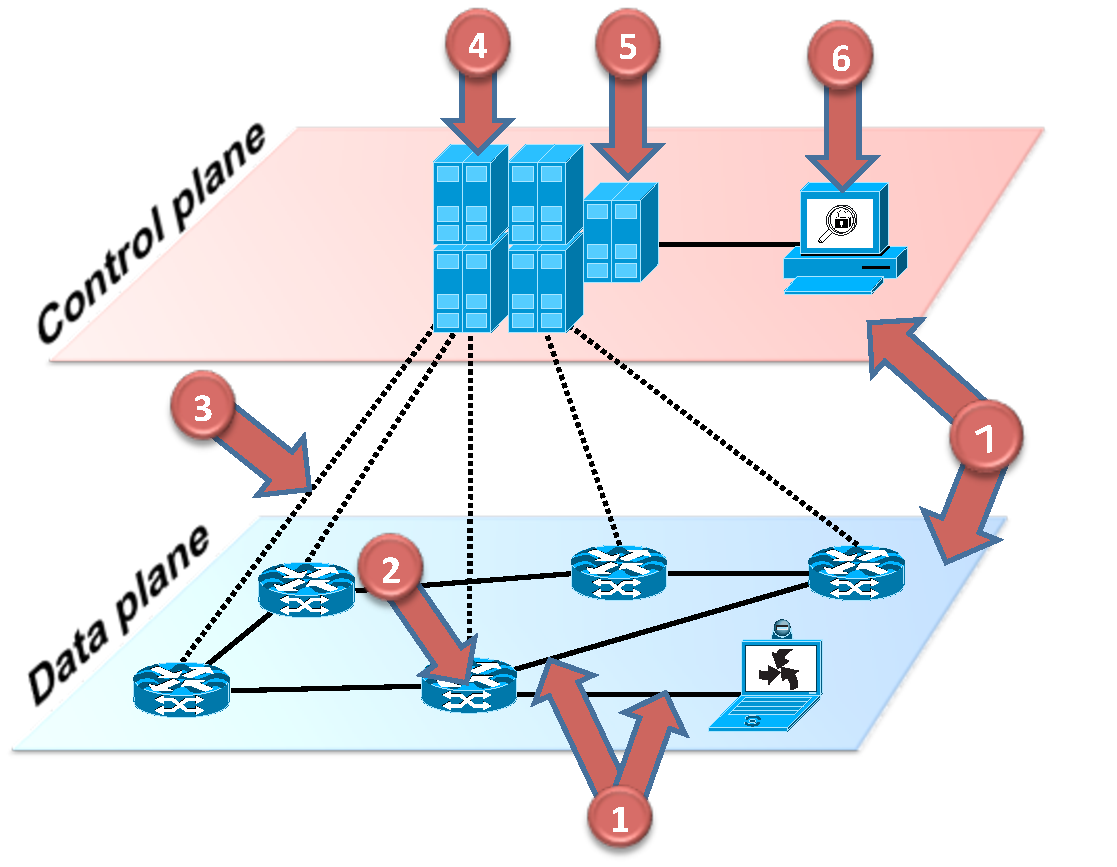
\includegraphics[width=0.85\columnwidth]{figures/fig9_sdn_threat_vectors.pdf}
\caption{Main threat vectors of SDN architectures}
\label{fig:threatvectorsmap}
\end{figure}

As can be observed in Table~\ref{tab:newandoldproblems}, threat vectors 3 to 5 are specific to SDN as they 
stem from the separation of the control and data planes and the consequent introduction of a new entity in 
these networks -- the logically centralized controller. The other vectors were already present 
in traditional networks. However, the impact of these threats could be larger than today -- or at least it 
may be expressed differently -- and as a consequence it may need to be dealt with differently.


{\renewcommand{\arraystretch}{1.4}
\begin{table}[!ht]
\caption{SDN specific vs. non-specific threats}
\label{tab:newandoldproblems}
\begin{center}
\footnotesize
%\rowcolors{1}{lightgray}{white}
\begin{tabularx}{\linewidth}{p{1.2cm}p{1.2cm}X}
\hline
\textbf{Threat vectors}  & \textbf{Specific to SDN?}  & \textbf{Consequences in software-defined networks} \\\hline
Vector 1      & no      & Open door for DDoS attacks.\\\hline
Vector 2      & no      & Potential attack inflation.\\\hline
Vector 3      & yes     & Exploiting logically centralized controllers.\\\hline
Vector 4      & yes     & Compromised controller may compromise the entire network.\\\hline
Vector 5      & yes     & Development and deployment of malicious applications on controllers. \\\hline
Vector 6      & no      & Potential attack inflation.\\\hline
Vector 7      & no      & Negative impact on fast recovery and fault diagnosis.\\
\hline
\end{tabularx}
\end{center}
\end{table}
}

OpenFlow networks are subject to a variety of security and dependability problems such as spoofing~\cite{kloti2013}, tampering~\cite{kloti2013}, 
repudiation~\cite{kloti2013}, information disclosure~\cite{kloti2013}, denial of service~\cite{kloti2013,shin2013,benton2013}, elevation of privileges~\cite{kloti2013}, \coloredtext{and the assumption that all applications are benign and will not affect SDN operation~\cite{shin2014}}.
The lack of isolation, protection, access control and stronger security recommendations\coloredtext{~\cite{wasserman2013,shin2013,porras2012,benton2013,shin2014}} are some of the reasons for these vulnerabilities.
We will explore these next.

%In the remaining of this section we introduce the main threat vectors of SDN and practical security issues of current OpenFlow-enabled networks. Additionally, we discuss some countermeasures that should be consider to address different security and dependability problems of SDN/OpenFlow.

\vspace{2mm}
\noindent \textit{OpenFlow security assessment}

\coloredtext{
%Currently, security is probably the Achilles' heel of SDN.
There is already a number of identified security issues in OpenFlow-enabled networks.
Starting from a STRIDE methodology~\cite{hernan2006}, it is possible to identify different attacks to OpenFlow-enabled networks.}
Table~\ref{tab:securitythreatsopenflow} summarizes these attacks (based on ~\cite{kloti2013}). 
For instance, information disclosure can be achieved through side channel attacks targeting the flow rule setup process. 
When reactive flow setup is in place, obtaining information about network operation is relatively easy.
An attacker that measures the delay experienced by the first packet of a flow and the subsequent can easily infer that the target network is a reactive SDN, and proceed with a specialized attack. 
This attack -- known as fingerprinting~\cite{shin2013} -- may be the first step to launch a DoS attack intended to exhaust the resources of the network, for example. 
If the SDN is proactive, guessing its forwarding rule policies is harder, but still feasible~\cite{kloti2013}. 
Interestingly, all reported threats and attacks affect all versions (1.0 to 1.3.1) of the OpenFlow specification. 
It is also worth emphasizing that some attacks, such as spoofing, are not specific to SDN. 
However, these attacks can have a larger impact in SDNs. 
For instance, by spoofing the address of the network controller, the attacker (using a fake controller) could  take over the control of the entire network. 
A smart attack could persist for only a few seconds, i.e., just the time needed to install special rules on all forwarding devices for its malicious purposes (e.g., traffic cloning). 
Such attack could be very hard to detect.

{\renewcommand{\arraystretch}{1.4}
\begin{table*}[!htp]
\caption{Attacks to OpenFlow networks.}
\label{tab:securitythreatsopenflow}
\begin{center}
\footnotesize
%\rowcolors{1}{lightgray}{white}
\begin{tabularx}{.85\textwidth}{ccX}
\hline
\textbf{Attack}  & \textbf{Security Property} & \textbf{Examples} \\\hline
\textbf{S}poofing & Authentication & MAC and IP address spoofing, forged ARP and IPv6 router advertisement\\\hline
\textbf{T}ampering & Integrity & Counter falsification, rule installation, modification affecting data plane.\\\hline
\textbf{R}epudiation & Non-repudiation & Rule installation, modification for source address forgery.\\\hline
\textbf{I}nformation disclosure & Confidentiality & Side channel attacks to figure out flow rule setup. \\\hline
\textbf{D}enial of service & Availability &  Flow requests overload of the controller. \\\hline
\textbf{E}levation of privilege & Authorization & Controller take-over exploiting implementation flaws. \\\hline
\end{tabularx}
\end{center}
\end{table*}
}

Taking counters falsification as another example, an attacker can try to guess installed flow 
rules and, subsequently, forge packets to artificially increase the counter.
Such attack would be specially critical for billing and load balancing systems, for instance.
A customer could be charged for more traffic than she in fact used, while a load balancing algorithm may take non-optimal decisions due to forged counters. 

Other conceptual and technical security concerns in OpenFlow networks include the lack of strong 
security recommendations for developers, the lack of TLS and access control support on most switch and controller 
implementations~\cite{wasserman2013}, the belief that TCP is enough because links are ``physically secure''~\cite{benton2013,wasserman2013}, the fact that many switches have listener 
mode activated by default (allowing the establishment of malicious TCP connections, for instance)~\cite{benton2013} or that flow table verification capabilities are harder to implement when TLS is not 
in use~\cite{wasserman2013,son2013}.
In addition, it is worth mentioning the high denial of service risk posed to centralized controllers~\cite{shin2013,son2013}, the vulnerabilities in the controllers themselves~\cite{son2013,kreutz2013}, \coloredtext{bugs and vulnerabilities in applications~\cite{Chandrasekaran2014_4}, targeted flooding attacks~\cite{jarraya2014}, insecure northbound interfaces that can lead to security breaches~\cite{jarraya2014}}, and the risk of resource depletion attacks~\cite{shin2013,benton2013}.
For instance, it has been shown that an attacker can easily compromise control plane communications through 
DoS attacks and launch a resource depletion attack on control platforms by exploiting a single  application such as a learning switch~\cite{benton2013,shin2013}.

\coloredtext{Another point of concern is the fact that current controllers, such as Floodlight, OpenDaylight, POX, and Beacon, have several security and resiliency issues~\cite{shin2014}.
Common application development problems (bugs), such as the sudden exit of an application or the continuous allocation of memory space, are enough to crash existing controllers.
On the security perspective, a simple malicious action such as changing the value of a data structure in memory can also directly affect the operation and reliability of current controllers.
These examples are illustrative that from a security and dependability perspective, there is still a long way to go.
}

\vspace{2mm}
\noindent \textit{Countermeasures for OpenFlow based SDNs}

Several countermeasures can be put in place to mitigate the security threats in SDNs.
Table~\ref{tab:countermeasuresthreats} summarizes a number of countermeasures that can be applied to different 
elements of an SDN/OpenFlow-enabled network. Some of these measures, namely rate limiting, event filtering, 
packet dropping, shorter timeouts, and flow aggregation, are already recommended in the most recent 
versions of the OpenFlow specification (version 1.3.1 and later). 
However, most of them are not yet supported or implemented in SDN deployments.

{\renewcommand{\arraystretch}{1.4}
\begin{table}[!htp]
\caption{Countermeasures for security threats in OpenFlow networks.}
\label{tab:countermeasuresthreats}
\begin{center}
\footnotesize
%\rowcolors{1}{lightgray}{white}
\begin{tabularx}{\columnwidth}{lX}
\hline
\multicolumn{1}{c}{\textbf{Measure}} & \multicolumn{1}{c}{\textbf{Short description}} \\\hline
Access control       & Provide strong authentication and authorization mechanisms on devices.  \\\hline
Attack detection     & Implement techniques for detecting different types of attacks. \\\hline
Event filtering         & Allow (or block) certain types of events to be handled by special devices. \\\hline
Firewall and IPS     & Tools for filtering traffic, which can help to prevent different types of attacks. \\\hline
Flow aggregation   & Coarse-grained rules to match multiple flows to prevent information disclosure and DoS attacks. \\\hline
Forensics support  & Allow reliable storage of traces of network activities to find the root causes of different problems.  \\\hline
Intrusion tolerance &  Enable control platforms to maintain correct operation despite intrusions. \\\hline
Packet dropping     & Allow devices to drop packets based on security policy rules or current system load. \\\hline
Rate limiting           & Support rate limit control to avoid DoS attacks on the control plane. \\\hline
Shorter timeouts  & Useful to reduce the impact of an attack that diverts traffic.  \\\hline
\end{tabularx}
\end{center}
\end{table}
}

Traditional techniques such as 
access control, attack detection mechanisms, event filtering (e.g.,  controller decides which asynchronous messages he is not going to accept), firewalls, and intrusion detection systems, can be used to mitigate the impact of or to avoid attacks.
They can be implemented in different devices, such as controllers, forwarding devices, middleboxes, and so forth.
Middleboxes can be a good option for enforcing security policies in an enterprise because they are (in general) more robust and special purpose (high performance) devices.
Such a strategy also reduces the potential overhead cause by implementing these countermeasures directly on controllers or forwarding devices.
However, middleboxes can add extra complexity to the network management, i.e., increase the OPEX at the cost of better performance.

Rate limiting, packet dropping, shorter timeouts and flow aggregations are techniques that can be applied on controllers and forwarding devices to mitigate different types of attacks, such as denial-of-service and information disclosure.
For instance, reduced timeouts can be used to mitigate the effect of an attack exploring the reactive operation mode of the network to make the controller install rules that divert traffic to a malicious machine. 
With reduced timeouts, the attacker would be forced to constantly generate a number of forged packets to avoid timeout expiration, making the attack more likely to be detected.
Rate limiting and packet dropping can be applied to avoid DoS attacks on the control plane or stop on-going attacks directly on the data plane by installing specific rules on the devices where the attacks is being originated.

Forensics and remediation encompass mechanisms such as secure logging, event correlation and consistent reporting. 
If anything wrong happens with the network, operators should be able to safely figure out the root cause of the problem and put the network to work on a secure operation mode as fast as possible.
Additionally, techniques to tolerate faults and intrusions, such as state machine replication~\cite{bolosky2011}, proactive-reactive recovery~\cite{sousa2010}, and diversity~\cite{garcia2013}, can be added to control platforms for increasing the robustness and security properties by automatically masking and removing faults.
Put differently, SDN controllers should be able to resist against different types of events (e.g., power outages, network disruption, communication failures, network partitioning) and attacks (e.g., DDoS, resource exhaustion)~\cite{kreutz2013,botelho2013}. 
One of the most traditional ways of achieving high availability is through replication. 
Yet, proactive-reactive recovery and diversity are two examples of crucial techniques that add value to the system for resisting against different kinds of attacks and failures (e.g., those exploring common vulnerabilities or caused by software aging problems).

Other countermeasures to address different threats and issues of SDN include enhancing the security and 
dependability of controllers, protection and isolation of applications\coloredtext{~\cite{sorensen2012,kreutz2013,porras2012,shin2014}}, trust management between controllers 
and forwarding devices~\cite{kreutz2013}, integrity checks of controllers and applications~\cite{kreutz2013}, forensics and remediation~\cite{sorensen2012,kreutz2013}, 
verification frameworks~\cite{chua2013,porras2012,korniak2011}, and resilient control planes~\cite{fonseca2012,korniak2011,kreutz2013,sorensen2012}.
Protection and isolation mechanisms should be part of any controller. Applications should be isolated from each other and from the controller. 
Different techniques such as security domains (e.g., kernel, security, and user level) and data access protection mechanisms should be put in place in order to avoid security threats from \manapps. 

Implementing trust between controllers and forwarding is another requirement for insuring that malicious elements 
cannot harm the network without being detected. 
An attacker can try to spoof the IP address of the controller and make switches connect to its own controller. 
This is currently the case since most controllers and switches only establish insecure TCP connections. 
Complementarly, integrity checks on controller and application software can help to ensure that safe code is being bootstrapped, which eliminates harmful software from being started once the system restarts. 
Besides integrity checks, other things such as highly specialized malware detection systems should be developed for SDN. 
Third-party \manapps should always be scanned for bad code and vulnerabilities because a malicious application represents a significant security threat to the network. 

It is worth mentioning that there are also other approaches for mitigating security threats in SDN, such as declarative languages to eliminate network 
protocol vulnerabilities~\cite{casey2013}. 
This kind of descriptive languages can specify semantic constraints, structural constraints and safe access properties of OpenFlow messages. 
Then, a compiler can use these inputs to find programmers' implementation mistakes on message operations. 
In other words, such languages can help find and eliminate implementation vulnerabilities of southbound specifications.

\coloredtext{Proposals providing basic security properties such as authentication~\cite{Toseef2014} and access control~\cite{Klaedtke2014-4} are starting to appear. 
C-BAS~\cite{Toseef2014} is a certificate-based AAA (Authentication, Authorization and Accounting) architecture for improving the security control on SDN experimental facilities.
%Such kind of solutions and developments of essential security mechanisms for SDNs are indeed required to foster the deployment of those network to the next level, i.e., wide spread adoption.
Solutions in the spirit of C-BAS can be made highly secure and dependable through hybrid system architectures, which combine different technologies and techniques from distributed systems, security, and fault and intrusion tolerance~\cite{Kreutz2014PRDC,Kreutz2014sodis,Verissimo2003ADS}.
%Furthermore, other proposals for access control are expected to appear as this is one of the major security issues of current SDN architectures.
}

\subsection{Migration and Hybrid deployments}
\label{sec:hybrid}

The promises by SDN to deliver easier design, operation and management of computer networks are endangered
by challenges regarding incremental deployability, robustness, and scalability. 
A prime SDN adoption challenge relates to organizational barriers that may arise due to the first (and second) order 
effects of SDN automation capabilities and ``layer/domain blurring''. 
Some level of human resistance is to be expected and may affect the decision and deployment processes of SDN, especially by those that may regard the 
control refactorization of SDN as a risk to the current chain of control and command, or even to their job security. 
This complex social challenge is similar (and potentially larger) to known issues between the transport and IP 
network divisions of service providers, or the system administrator, storage, networking, and security teams 
of enterprise organizations. Such a challenge is observable on today's virtualized data centers, through the shift 
in role and decision power between the networking and server people. Similarly, the development and operations (DevOps) movement has caused a shift in the locus of influence, not only 
on the network architecture but also on purchasing, and this is an effect that SDN may exacerbate. These changes in role and power causes a second order effect on the sales division of vendors that are required to adapt accordingly. 


Pioneering SDN operational deployments have been mainly greenfield scenarios and/or tightly controlled single 
administrative domains. Initial roll-out strategies are mainly based on virtual switch overlay models or 
OpenFlow-only network-wide controls. However, a broader adoption of SDN beyond data center silos -- and 
between themselves -- requires considering the interaction and integration with legacy control planes providing 
traditional switching; routing; and operation, administration, and management (OAM) functions. Certainly, 
rip-and-replace is not a viable strategy for the broad adoption of new networking technologies.

Hybrid networking in SDN should allow deploying OpenFlow for a subset of all flows only, enable OpenFlow on 
a subset of devices and/or ports only, and provide options to 
interact with existing OAM protocols, legacy devices, and neighboring domains. As in any technology transition 
period where fork-lift upgrades may not be a choice for many, migration paths are critical for 
adoption.

Hybrid networking in SDN spans several levels. The Migration Working Group of the ONF is tackling the scenario where hybrid switch architectures and hybrid (OpenFlow and non-OpenFlow) devices 
co-exist. Hybrid switches can be configured to behave as a legacy switch or as an OpenFlow switch and, in some 
cases, as both simultaneously. This can be achieved, for example, by partitioning the set of ports of a switch, 
where one subset is devoted to OpenFlow-controlled networks, and the other subset to legacy networks. For these 
subsets to be active at the same time, each one having its own data plane, multi-table support at the forwarding 
engine (e.g., via TCAM partitioning) is required. Besides port-based partitioning, it is also possible to rely 
on VLAN-based (prior to entering the OpenFlow pipeline) or flow-based partitioning using OpenFlow matching and 
the \texttt{LOCAL} and/or \texttt{NORMAL} actions to redirect packets to the legacy pipeline or the switch's 
local networking stack and its management stack. Flow-based partitioning is the most flexible option, as it 
allows each packet entering a switch to be classified by an OpenFlow flow description and treated by the 
appropriate data plane (OpenFlow or legacy).

There are diverse controllers, such as OpenDaylight~\cite{opendaylight2013}, HP VAN SDN~\cite{hp2013-1}, and OpenContrail~\cite{junipernetworks2013-1}, that have been designed to integrate current non-SDN technologies (e.g., SNMP, PCEP, BGP, NETCONF) with SDN interfaces such as OpenFlow and OVSDB.
Nonetheless, controllers such as ClosedFlow~\cite{Hand2014_4} have been recently proposed with the aim of introducing SDN-like programming capabilities in traditional network infrastructures, making the integration of legacy and SDN-enabled networks a reality without side effects in terms of programmability and global network control.
ClosedFlow is designed to control legacy Ethernet devices (e.g., Cisco 3550 switches with a minimum IOS of 12.2 SE) in a similar way an OpenFlow controller allows administrators to control OpenFlow-enabled devices.
More importantly, ClosedFlow does not impose any change on the forwarding devices. 
It only takes advantage of the existing hardware and firmware capabilities to mimic an SDN control over the network, i.e., allow dynamic and flexible programmability in the data plane.
The next step could be the integration of controllers like ClosedFlow and OpenFlow-based controllers, promoting interoperability among controllers and a smooth transition from legacy infrastructures to SDN-enabled infrastructure with nearly all the capabilities of a clean-slate SDN-enabled infrastructure.

Furthermore, controllers may have to be separated into distinct peer domains for different reasons, such as scalability, technology, controllers from different vendors, controllers with different service functionality, and diversity of administrative domains~\cite{ONF2014SDNarch}.
Controllers from different domains, or with distinct purposes, are also required to be backwards compatible either by retrofitting or extending existing multi-domain protocols (e.g. BGP) or by proposing new SDN-to-SDN protocols (aka east/westbound APIs).
%These are some of the challenges not yet completely addressed.

Some efforts have been already devoted to the challenges of migration and hybrid SDNs. RouteFlow~\cite{rothenberg2012-1} implements an IP level control plane on top of an OpenFlow 
network, allowing the underlying devices to act as IP routers under different possible arrangements. \coloredtext{The Cardigan project~\cite{stringer2013,floss-meets-sdn} has deployed RouteFlow at a live Internet eXchange now for over a year.  
LegacyFlow~\cite{rothenberg2014} extends the OpenFlow-based controlled network to embrace non-OpenFlow nodes. 
There are also some other early use cases on integrating complex legacy system such as DOCSIS~\cite{Fuentes2014}, Gigabit Ethernet passive optical network and DWDM ROADM (Reconfigurable Optical Add/Drop Multiplexer)~\cite{Parniewicz2014,Belter2014}.}
The common 
grounds of these pieces of work are (1) considering hybrid as the coexistence of traditional environments of 
closed vendor's routers and switches with new OpenFlow-enabled devices; (2) targeting the interconnection of 
both control and data planes of legacy and new network elements; and (3) taking a controller-centric approach, 
drawing the hybrid line outside of any device itself, but into the controller application space.

Panopticon~\cite{levin2014} defines an architecture and methodology to consistently implement 
SDN inside enterprise legacy networks through network orchestration under strict budget constraints. The proposed 
architecture includes policy configurations, troubleshooting and maintenance tasks establishing transitional networks 
(SDN and legacy) in structures called Solitary Confinement Trees (SCTs), where VLAN IDs are efficiently used by 
orchestration algorithms to build paths in order to steer traffic through SDN switches. Defying the partial SDN 
implementation concept, they confirm that this could be a long-term operational strategy solution for enterprise 
networks.

HybNET~\cite{lu2013} presents a network management framework for
hybrid OpenFlow-legacy networks. It provides a common centralized
configuration interface to build virtual networks using VLANs. An
abstraction of the physical network topology is taken into account by
a centralized controller that applies a path finder mechanism, in
order to calculate network paths and program the OpenFlow switches via
REST interfaces and legacy devices using NETCONF~\cite{enns2011-1}.

\coloredtext{More recently, frameworks such as ESCAPE~\cite{Csoma2014}  and its extensions have been proposed to provide multi-layer service orchestration in multi-domains.
Such frameworks combine different tools and technologies such as Click~\cite{morris1999}, POX~\cite{mccauley2012}, OpenDaylight~\cite{opendaylight2013} and NETCONF~\cite{enns2011-1}.
In other words, those frameworks integrate different SDN solutions with traditional ones.
Therefore, they might be useful tools on the process of integrating or migrating legacy networking infrastructure to SDN.

Other hybrid solutions starting to emerge include Open Source Hybrid IP/SDN (OSHI)~\cite{salsano2014oshi}. 
OSHI combines Quagga for OSPF routing and SDN capable switching devices (e.g., Open vSwitch) on Linux to provide  backwards compatibility for supporting incremental SDN deployments, i.e., enabling interoperability with non-OF forwarding devices in carrier-grade networks.
%It is also worth mentioning that the current version of the OSHI node offers support to three different environments, VirtualBox, Mininet  and the OFELIA testbed~\cite{sune2014ofelia}.
}


While full SDN deployments are straightforward only in some green field deployments such as data center networks or by 
means of an overlay model approach, hybrid SDN approaches represent a very likely deployment model 
that can be pursued by different means, including~\cite{vissicchio2014}:

\begin{itemize}
\item Topology-based hybrid SDN: Based on a topological separation of the nodes controlled by traditional and SDN 
paradigms. The network is partitioned in different zones and each node belongs to only one zone. 
\item Service-based hybrid SDN: Conventional networks and SDN provide different services, where overlapping nodes, 
controlling a different portion of the FIB (or generalized flow table) of each node. Examples include network-wide 
services like forwarding  that can be based on legacy distributed control, while SDN provides edge-to-edge services 
such as enforcement of traffic engineering and access policies, or services requiring full traffic visibility 
(e.g., monitoring).
\item Class-based hybrid SDN: Based on the partition of traffic in classes, some controlled by SDN and the remaining 
by legacy protocols. While each paradigm controls a disjoint set of node forwarding entries,  each paradigm is 
responsible for all network services for the assigned traffic classes. 
\item Integrated hybrid SDN: A model where SDN is responsible for all the network services, and
uses traditional protocols (e.g., BGP) as an interface to node FIBs. For example, it can control forwarding
paths by injecting carefully selected routes into a routing system or adjusting protocol settings (e.g., IGP weights). 
Past efforts on RCPs~\cite{caesar2005} and the ongoing efforts within ODL~\cite{opendaylight2013} can be considered 
examples of this hybrid model.
\end{itemize}

In general, benefits of hybrid approaches include enabling flexibility (e.g., easy match on packet fields for 
middleboxing) and SDN-specific features (e.g., declarative management interface) while partially keeping the inherited 
characteristics of conventional networking such as robustness, scalability, technology maturity, and low deployment 
costs. On the negative side, the drawbacks of hybridization include the need for ensuring profitable interactions 
between the networking paradigms (SDN and traditional) while dealing with the heterogeneity that largely depends on 
the model.

Initial trade-off analyses~\cite{vissicchio2014} suggest that the combination of centralized and distributed paradigms may provide 
mutual benefits. However, future work is required to devise techniques and interaction mechanisms that maximize 
such benefits while limiting the added complexity of the paradigm coexistence.


%\subsection{SDN for telecom and cloud providers}

\subsection{Meeting carrier-grade and cloud requirements}

A number of carrier-grade infrastructure providers (e.g., NTT, AT\&T, Verizon, Deutsche Telekom) are at the core of the SDN community with the ultimate goal of solving their long standing networking problems.
%One of the forefront runners (and early SDN adopter) is NTT, already taking advantage o this new paradigm to provide new on-demand network provisioning models. 
\coloredtext{In the telecom world, NTT can be considered one of the forefront runners in terms of investing in the adoption and deployment of SDN in all kinds of network infrastructures, from backbone, data center, to edge customers~\cite{Reinecke2014}. In 2013, NTT launched an SDN-based, on-demand elastic provisioning platform of network resources (e.g., bandwidth) for HD video broadcasters~\cite{bernier2013}.
%Similarly to self driving cars, NTT is fostering the development of a network that drives itself, i.e., a central intelligence that can automate most of the traditional tasks and provide autonomic functions and services to the network.
}
Similarly, as a global cloud provider with data centers spread across the globe~\cite{nttdata2014}, the same company launched a similar service for its cloud customers, who are now capable of taking advantage of dynamic networking 
provisioning intra- and inter-data centers~\cite{wagner2014}.
AT\&T is another telecom company that is investing heavily in new services, such as user-defined network clouds, that 
take advantage of recent developments in NFV and SDN~\cite{atandtinc.2014}.
\coloredtext{As we mentioned before, SDN and NFV are complementary technologies that can be applicable to different types of networks, from local networks and data centers to transport networks~\cite{Haleplidis2014_4,onf2014-1,Cerrato2014-1,Xia2014_4,haleplidis2014sdnnfv,gemberjacobson2014}.
Recently, several research initiatives have worked towards combining SDN and NFV through Intel's DPDK, a set of libraries and drivers that facilitates the development of network-intensive applications and allows the implementation of fine-grained network functions~\cite{Cerrato2014}. 
Early work towards service chaining have been proposed by combining SDN and NFV technologies~\cite{Ruckert2014,Blendin2014,Skoldstrom2014,Jamjoom2014_4,john2013nsc}, and studies around the ForCES's~\cite{doria2010} applicability to SDN-enhanced NFV have also come to light~\cite{Haleplidis2014_4}.}
%, and so forth~\cite{onf2014-1}.}
These are some of the early examples of the opportunities SDNs seem to bring to telecom and cloud providers. 

Carrier networks are using the SDN paradigm as the technology means for solving a number of long standing problems. 
%in an easier way, such as inter-data center over-provisioned router links, static allocation 
%of circuit-switched links, isolation of operation by network layers, separated management of L3/L2 and L1 
%infrastructure (which causes lots of extra costs by requiring multiple sets of  people  to  operate them - engineering,    planning, provisioning), fine-grained QoS, and network virtualization. 
Some of these efforts include 
new architectures for a smooth migration from the current mobile core infrastructure to SDN~\cite{pentikousis2013}, and techno-economic models for virtualization of these networks~\cite{naudts2012,onfsolutionbrief2013};  
carrier-grade OpenFlow virtualization schemes~\cite{skoldstrom2013,koponen}, including virtualized broadband access infrastructures~\cite{gharakheili2013}, techniques that are allowing the offer of network-as-a-service~\cite{pacnet2013}; 
\coloredtext{programmable GE-PON and DWDM ROADM~\cite{Parniewicz2014,Belter2014,Belter2014-1,Clegg2014}; large-scale inter-autonomous systems (ASs) SDN-enabled deployments~\cite{bennesby2012inter};}
flexible control of network resources~\cite{corporation2012}, including offering MPLS services using an SDN approach~\cite{das2011};
and the investigation of novel network architectures, from proposals to separate the network edge from the core~\cite{casado2012,6786608}, with the latter forming the fabric that transports packets as defined by an intelligent edge, to software-defined Internet exchange points~\cite{feamster2013,stringer2013}.

\coloredtext{Use-case analysis~\cite{Devlic2012} of management functions required by carrier networks have identified a set of requirements and existing limitations in the SDN protocol toolbox. 
For instance, it has been pinpointed that OF-Config~\cite{OFCONFIG} needs a few extensions in order to meet the carrier requirements, such as physical resource discovery, logical link configuration, logical switch instantiation, and device and link OAM configuration~\cite{Devlic2012}.
%Some of these extensions imply also modifications on the OpenFlow protocol itself.
Similarly, OpenFlow extensions have also been proposed to realize packet-optical integration with SDN~\cite{shirazipour2012}.
In order to support SDN concepts in large-scale wide area networks, different extensions and mechanisms are required, both technology-specific (e.g., MPLS BFD) and technology agnostic, such as: resiliency mechanisms for surviving link failures~\cite{Adrichem2014}, failures of controller or forwarding elements; solutions for integrating residential customer services in different forms (i.e., support also current technologies); new energy-efficient networking approaches; QoS properties for packet classification, metering, coloring, policing, shaping and scheduling; and multi-layer aspects outlining different stages of packet-optical integration~\cite{John2014_4,John2014split,shirazipour2012}.
}
%
%\coloredtext{Research efforts on resilient OpenFlow networksusing group tables for fast failover and leveraging BFD like failure detection suggest that SDN can achieve stringent telecom requirements, such as sub 50 ms latency path restoration.}


SDN technology also brings new possibilities for cloud providers.
By taking advantage of the logically centralized control of network resources~\cite{hong2013,jain2013-1} it is possible to simplify and optimize network management of data centers and achieve:
(i) efficient intra-datacenter networking, including fast recovery mechanisms for the  data and control planes~\cite{sharma2013-1,staessens2011,sharma2013}, adaptive traffic engineering with minimal modifications to DCs networks~\cite{benson2011mTE}, simplified fault-tolerant routing~\cite{mysore2009}, performance isolation~\cite{greenberg2009}, and easy and efficient resource migration (e.g., of VMs and virtual networks)~\cite{sharma2013-1};
(ii) improved inter-datacenter communication, including the ability to fully utilize the expensive high-bandwidth links without impairing quality of service~\cite{jain2013-1,sadasivarao2013};
(iii) higher levels of reliability (with novel fault management mechanisms, etc.)~\cite{mysore2009,staessens2011,sharma2013-1,Adrichem2014}; and 
(iv) cost reduction by replacing complex, expensive hardware by simple and cheaper forwarding devices~\cite{tanner2013,jain2013-1}.



Table~\ref{tab:carriergradeneeds} summarizes some of the carrier-grade network and cloud infrastructure providers' requirements.
In this table we show the current challenges and what is to be expected with SDN.
As we saw before, some of the expectations are already becoming a reality, but many are still open issues.
What seems to be clear is that SDN represents an opportunity for telecom and cloud providers, in providing flexibility, cost-effectiveness, and easier management of their networks.

{\renewcommand{\arraystretch}{1.4}
\begin{table*}[t!]
\caption{Carrier-grade and cloud provider expectations \& challenges}
\label{tab:carriergradeneeds}
\newcommand{\firstcolumnwidth}{2.5cm} 
\begin{center}
\footnotesize
\begin{tabularx}{0.99\textwidth}{p{\firstcolumnwidth}p{6cm}X}
\hline
\textbf{What} & \textbf{Currently} & \textbf{Expected with SDN} \\\hline
\multirow{8}{*}{\begin{minipage}{\firstcolumnwidth}Resource Provisioning\end{minipage}} 
                     & Complex load balancing configuration. & Automatic load balancing reconfiguration.~\cite{elby2012,jain2013-1} \\\cline{2-3}
		    & Low virtualization capabilities across hardware platforms & NFV for virtualizing network functionality across hardware appliances.~\cite{tanner2013,atandtinc.2014} \\\cline{2-3}
		    & Hard and costly to provide new services. & Create and deploy new network service quickly.~\cite{tanner2013,atandtinc.2014}\\\cline{2-3}
                     & No bandwidth on demand. & Automatic bandwidth on demand.~\cite{onfsolutionbrief2013} \\\cline{2-3}
                     & Per network element scaling. & Better incremental scaling.~\cite{elby2012,staessens2011} \\\cline{2-3}
		    & Resources statically pre-provisioned. & Dynamic resource provisioning in response to load.~\cite{elby2012,jain2013-1,tanner2013,naudts2012,hong2013} \\
\hline
\multirow{4}{*}{\begin{minipage}{\firstcolumnwidth}Traffic Steering\end{minipage}} 
                     & All traffic is filtered. & Only targeted traffic is filtered.~\cite{elby2012} \\\cline{2-3}
                     & Fixed only. & Fixed and mobile.~\cite{elby2012} \\\cline{2-3}
                     & Per network element scaling. & Better incremental scaling. ~\cite{naudts2012,staessens2011}\\\cline{2-3}
                     & Statically configured on a per-device basis. & Dynamically configurable.~\cite{jain2013-1,onfsolutionbrief2013,anwer2013} \\
\hline
\multirow{4}{*}{\begin{minipage}{\firstcolumnwidth}Ad Hoc Topologies\end{minipage}}   
                     & All traffic from all probes collected. & Only targeted traffic from targeted probes is collected. \\\cline{2-3}
                     & Massive bandwidth required. & Efficient use of bandwidth.~\cite{jain2013-1,onfsolutionbrief2013} \\\cline{2-3}
                     & Per network element scaling. & Better incremental scaling.~\cite{elby2012,onfsolutionbrief2013} \\\cline{2-3}
                     & Statically configured. & Dynamically configured.~\cite{elby2012,gerlach2013,bernier2013} \\
\hline
\multirow{7}{*}{\begin{minipage}{\firstcolumnwidth}Managed Router\\ Services\end{minipage}}   
                     & Complex configuration, management and upgrade. & Simplified management and upgrade.~\cite{jain2013-1,elby2012,tanner2013,onfsolutionbrief2013,staessens2011} \\\cline{2-3}
                     & Different kinds of routers, such as changeover (CO). & No need for CO routers, reducing aggregation costs.~\cite{elby2012,tanner2013,naudts2012} \\\cline{2-3}
                     & Manual provisioning. & Automated provisioning.~\cite{elby2012,onfsolutionbrief2013,anwer2013} \\\cline{2-3}
                     & On-premises router deployment. & Virtual routers (either on-site or not).~\cite{onfsolutionbrief2013,elby2012,naudts2012} \\\cline{2-3}
                     & Operational burden to support different equipments. & Reduced technology obsolescence.~\cite{naudts2012} \\\cline{2-3}
                     & Router change-out as technology or needs change. & Pay-as-you grow CAPEX model.~\cite{naudts2012} \\\cline{2-3}
                     & Systems complex and hard to integrate. & Facilitates simplified system integrations.~\cite{elby2012,tanner2013,gerlach2013}\\\hline
\multirow{2}{*}{\begin{minipage}{\firstcolumnwidth}Revenue Models\end{minipage}}   
                     & Fixed long term contracts. & More flexible and on-demand contracts.~\cite{onfsolutionbrief2013,corporation2012}\\\cline{2-3}
                     & Traffic consumption. & QoS metrics per-application.~\cite{onfsolutionbrief2013,staessens2011,staessens2011,velasco2013} \\
\hline
\multirow{4}{*}{\begin{minipage}{\firstcolumnwidth}Middleboxes \\Deployment \& \\Management\end{minipage}}   
                     & Composition of services is hard to implement. & Easily expand functionality to meet the infrastructure needs.~\cite{tanner2013}\\\cline{2-3}
                     & Determine where to place middleboxes a priori (e.g., large path inflation problems). & Dynamic placement using shortest or least congested path. ~\cite{qazi2013-1,velasco2013,gerlach2013} \\\cline{2-3}
                     & Excessive over-provisioning to anticipate demands. & Scale up to meet demands, and scale down to conserve resources (elastic middleboxes).~\cite{elby2012,naudts2012} \\
\hline
\multirow{3}{*}{\begin{minipage}{\firstcolumnwidth}Other Issues\end{minipage}}   
                     & Energy saving strategies are hard to implement. & Flexible and easy to deploy energy saving strategies.~\cite{staessens2011}\\\cline{2-3}
                     & Complex and static control and data plane restoration techniques. & Automated and flexible restoration techniques for both control and data plane.~\cite{staessens2011}\\\cline{2-3}
\hline
\end{tabularx}
\end{center}
\end{table*}
}

%For instance, telecom providers such as Verizon 
%~\cite{elby2012} foresee several advantages and improvements for carrier-grade network infrastructures.
%Examples include implementation of network functions on COTS hardware, virtualization of network functions,
%application and service aware routing, orchestration of network and cloud resources,
%added efficiency on the network, and on-demand virtual network resource provisioning. 
%Use-cases range from dynamic resource provisioning, automatic load balancing reconfiguration, traffic steering (e.g., targeted traffic 
%filtering, incremental network scaling per device), ad-hoc network topologies with QoS assurance, to integration 
%of new functions in the network.

\subsection{SDN: the missing piece towards Software-Defined Environments}

The convergence of different technologies is enabling the emergence of fully programmable IT infrastructures.
It is already possible to dynamically and automatically configure or reconfigure the entire IT stack, from the network infrastructure up to the applications, to better respond to workload changes.
Recent advances makes on-demand provisioning of resources possible, at nearly all infrastructural layers.
The fully automated provisioning and orchestration of IT infrastructures as been recently named Software-Defined Environments (SDEs)~\cite{racherla2014,li2014}, by IBM.
This is a novel approach that is expected to have significant potential in simplifying IT management, optimizing the use of the infrastructure, reduce costs, 
and reduce the time to market of new ideas and products.
In an SDE, workloads can be easily and automatically assigned to the appropriate IT resources based on application characteristics, security and service level policies, and the best-available resources to deliver continuous, dynamic optimization and reconfiguration to address infrastructure issues in a rapid and responsive manner.
Table~\ref{tab:TraditionalAndSDE} summarizes the traditional approaches and some of the key features being enabled 
by SDEs~\cite{alba2014,arnold2014}.

{\renewcommand{\arraystretch}{1.4}
\begin{table*}[t!]
\caption{SDE pushing IT to the next frontier}
\label{tab:TraditionalAndSDE}
\newcommand{\firstcolumnwidth}{3.2cm} 
\begin{center}
\footnotesize
\begin{tabularx}{0.99\textwidth}{XX}
\hline
\textbf{Traditionally} & \textbf{Expected with SDEs} \\\hline
IT operations manually map the resources for apps for software deployment.  & Software maps resources to the workload and deploys the workload. \\\hline
Networks are mostly statically configured and hard to change.  & Networks are virtualized and dynamically configured on-demand. \\\hline
Optimization and reconfiguration to reactively address issues are manual.  & Analytics-based optimization and reconfiguration of infrastructure issues. \\\hline
Workloads are typically manually assigned to resources.  & Workloads are dynamically assigned. \\\hline
%\\\hline
\end{tabularx}
\end{center}
\end{table*}
}

In an SDE the workloads are managed independently of the systems and underlying infrastructure, i.e., are not tied to a specific technology or vendor~\cite{li2014,racherla2014}.
Another characteristic of this new approach is to offer a programmatic access to the environment as a whole, selecting the best available resources based on the current status of the infrastructure, and enforcing the policies defined.
In this sense, it shares much of the philosophy of SDN.
Interestingly, one of the missing key pieces of an SDE was, until now, Software-Defined Networking.

The four essential building blocks of an SDE~\cite{li2014,racherla2014,arnold2014} are:

\begin{itemize}
\item Software-Defined Networks (SDN)~\cite{dixon2014,ibmsystemsandtechnologygroup2014},
\item Software-Defined Storage (SDS)~\cite{alba2014},
\item Software-Defined Compute (SDC)~\cite{racherla2014}, and 
\item Software-Defined Management (SDM)~\cite{ibmsystems2014}.
\end{itemize}

In the last decade the advances in virtualization of compute and storage, together with the availability of sophisticated cloud orchestration tools have enabled SDS, SDC and SDM.
These architectural components have been widely used by cloud providers and for building IT infrastructures in different enterprise environments.
However, the lack of programmable network control has so far hindered the realization of a complete Software-Defined Environment.
SDN is seen as the technology that may fill this gap, as attested by the emergence of cloud-scale network virtualization platforms based on this new paradigm~\cite{koponen}.

%SDEs are becoming, at a relatively fast pace, key orchestration systems to drive IT management to the next 
%level, changing the long standing essential static or manually setup of the infrastructure and systems to 
%accommodate diverse and dynamic workloads. 
%Traditionally, IT infrastructures have been quite complex and hard to manage and evolve, and in particular 
%the network. For instance, workloads are typically manually assigned to resources, networks are mostly statically 
%configured and hard to change, IT operations manually map the resources for applications for software deployment, optimization and reconfiguration to reactively address issues are also manual.


%Traditionally:
%workloads are typically manually assigned to resources;
%networks are mostly statically configured and hard to change;
%IT operations manually map the resources for applications for software deployment;
%optimization and reconfiguration to reactively address issues are also manual.
%
%with SDEs:
%workloads are dynamically assigned;
%networks are virtualized and dynamically configured in an on-demand fashion;
%Software maps resources to the workload and deploys the workload;
%Analytics-based optimization and reconfiguration address infrastructure issues.
%

% Figure: SDE-enabled IT infrastructure overview.
\begin{figure}[ht!]
\centering
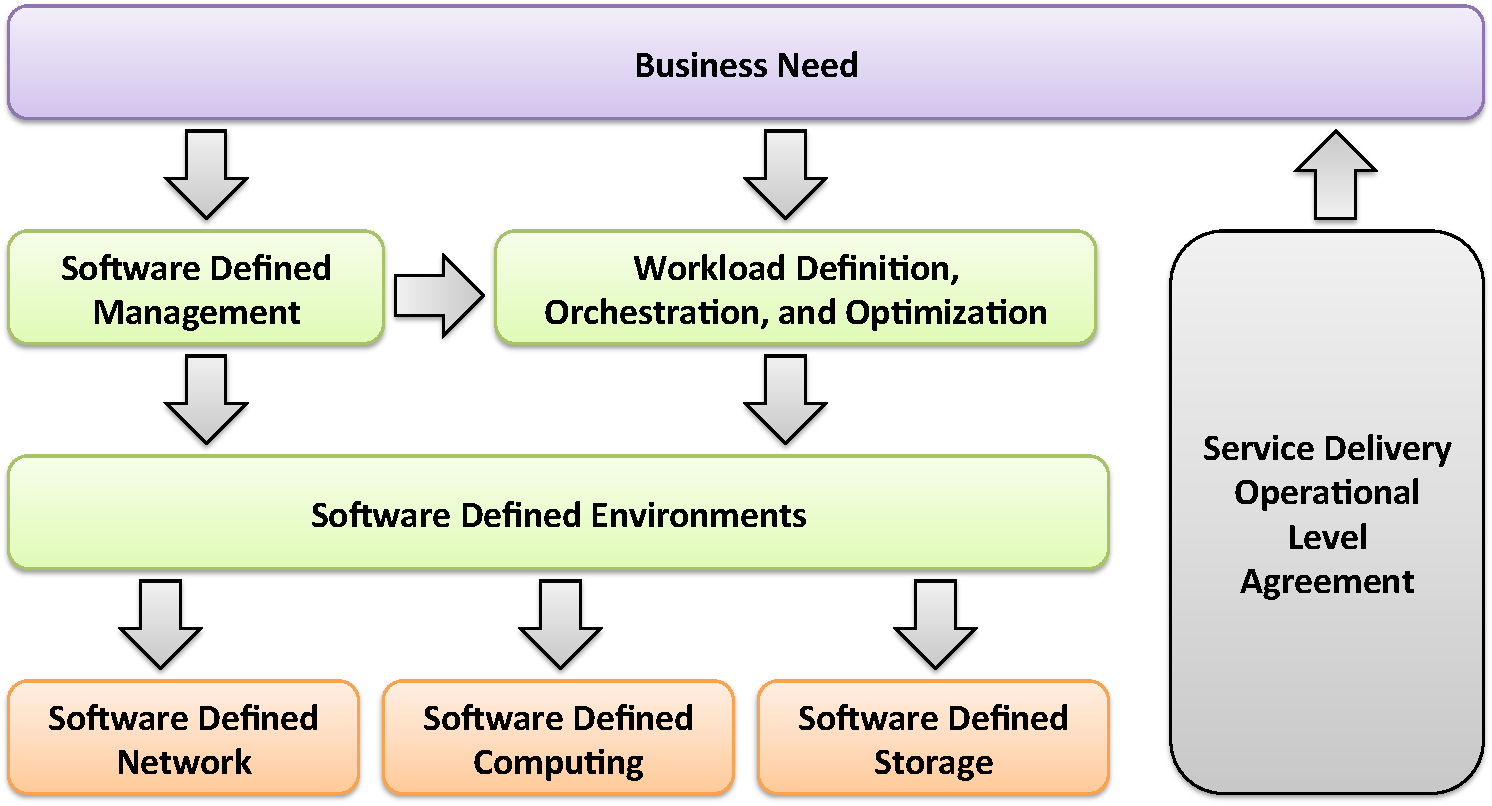
\includegraphics[width=0.95\columnwidth]{figures/fig10_sde_enabled_IT.pdf}
\caption{Overview of an IT infrastructure based on a SDE.}
\label{fig:SDEenabledIT}
\end{figure}


The IBM SmartCloud Orchestrator is one of the first examples of an SDE~\cite{li2014,racherla2014}.
It integrates compute, storage, management and networking in a structured way.
Figure~\ref{fig:SDEenabledIT} gives a simplified overview of an SDE, by taking the approach developed by IBM as its basis.
The main idea of an SDE-based infrastructure is that the business needs that define the workloads trigger the reconfiguration of the global IT infrastructure (compute, storage, network). 
This is an important step towards a more customizable IT infrastructure that focuses on the business requirements rather than on the limitations of the infrastructure itself.


% FIXME: XXXXX

%It is worth to emphasize that SDN plays a major key role in enabling SDEs.
%Currently, vendors take advantage of the flexibility and programmability provided by controllers on the control plane to optimize network resources utilization to achieve high performance and competitive advantages. 
%The forwarding devices-based control plane paradigm gives network administrators a first opportunity to fix the bleeding need of increasing data flow efficiency across the network as a whole.

%Nowadays, with SDN, instead of thinking the network as a monolithic, complex and hard to evolve infrastructure, 
%one can now think about the network as a software platform. The evolution of the network is now limited mostly 
%by the software (e.g., applications), i.e., network functions and protocols are driven by fast evolving software 
%components, which provides a greater flexibility and a very fast pace of evolution when compared to traditional
%networks. Moreover, it is much easier to integrate the network control with higher-level software stacks, such 
%as hypervisors and cloud orchestration. Figure~\ref{fig:SDNandSDE} illustrates how SDN can fit in the new 
%software enabled IT infrastructures~\cite{racherla2014}.

% Figure: relationship of SDN and the SDE.
%\begin{figure}[ht!]
%\centering
%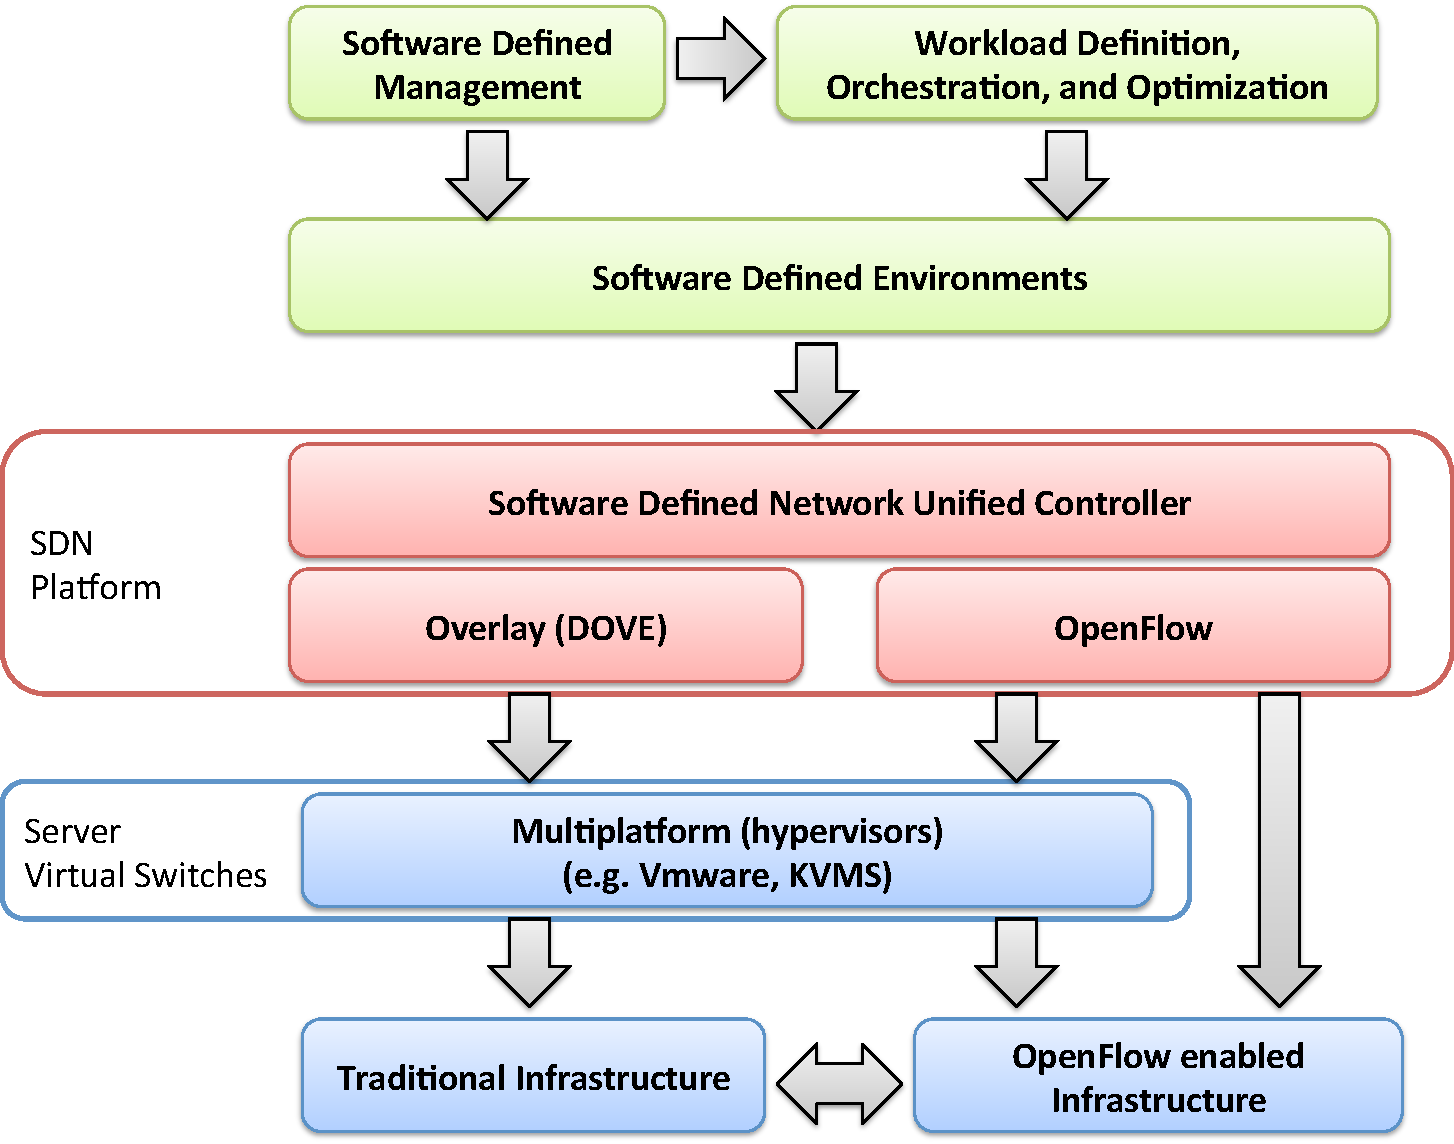
\includegraphics[width=0.95\columnwidth]{figures/fig11_sde_and_sdn.pdf}
%\caption{SDN completing the puzzle of an SDE.}
%\label{fig:SDNandSDE}
%\end{figure}

%The SDN Unified Controller represents IBM's approach for using SDN as one of the essential building blocks 
%for the next generation of SDEs. There are different concerns and driving forces of SDN into this new world 
%of SDEs. First, SDN is an obvious useful tool for helping to consolidate and virtualize server platforms and 
%network resources. Some of the main trade-offs in merging server and network virtualization is directly related 
%with the enforcement of security policies. On one hand, we have several driving forces toward highly 
%efficient systems. On the other hand, we need to guarantee security isolation and QoS guarantees for the 
%virtual networks of tenants. SDN helps tackle these issues by making it possible for security control 
%enforcement elements to be placed in the right place, i.e., where it makes more sense in terms of computing 
%needs and network flows. Second, cost reduction has always been one of the major forces that is driven by the 
%global economy, always putting some sort of stress on the enterprise IT budgets. Therefore, IT projects that 
%are not capable of demonstrating the added-value for the business have day-after-day less chance to succeed.
%SDN can be used as a key tool to demonstrate that business can now experience a decreasing time to market thanks 
%to (1) dynamic and fast resource provisioning mechanisms, (2) a reduced capital expenditure by shifting the costs 
%from intelligent and expensive hardware devices to software running on top of commodity server platforms, and 
%(3) reduced overall operational expenses through a global blueprint of what is running on the infrastructure 
%without the hassle of having to manage diverse systems commonly controlled by specific, proprietary and complex 
%protocols and tools. Put differently, SDN makes enterprise LANs shift from locked-in and complex solutions to 
%a model where the forwarding devices functionality is a common and simple enough industry accepted standard to 
%make multi-vendor networks an attractive solution for clients.

%It is also worth emphasizing that in this new virtualized and highly integrated world, it is important that 
%data center professionals have a broad knowledge. These professionals have now to know about a variety of 
%technologies and new concepts such as hypervisors, storage, computing virtualization, storage virtualization, 
%network virtualization, software-defined networks, security, elasticity of computing, storage and networking 
%resources, full environment migration, and so forth. Most importantly, IT sections of enterprise cannot be organized 
%anymore into independent silos. The interdependencies between the different infrastructure layers, technologies 
%and resources have reached their peak. For instance, SDEs are driving a major change in computing and networking 
%infrastructure, where applications at the top level start to define the computing, storage and networking 
%resources. Therefore, it is more than critical to have a global and collective view of what is available in 
%the infrastructure for business applications and systems. Naturally, it implies in new skills and 
%multidisciplinary approaches, which are not yet a common case in IT organizations. In fact, many times, there 
%is some resistance between different teams (e.g., security and network infrastructure, development and security, 
%development and network infrastructure, IT business requirements and IT infrastructure teams and/or providers) 
%to interact and be flexible enough to understand and try out smart solution to a variety of interesting, and 
%sometimes complicated, problems.

%It seems clear that the key pieces for SDE can finally be put together. More importantly, 
%the missing piece of this complex puzzle, SDN, is finally under a fast pace development and evolution. However, 
%there is still a long way and many interesting challenges in designing, implementing and deploying SDEs. IBM took 
%the first step in this direction by providing commercial products capable of delivering some of the exciting 
%features of these new dynamically programmable environments, focusing always on the business and application 
%requirements, rather than putting IT as a barrier to the business evolution.